\documentclass{ZJUthesis}
\hypersetup{colorlinks=false}
\begin{document}
%%%%%%%%%%%%%%%%%%%%%%%%%%%%%
%% 正文字体设定
%%%%%%%%%%%%%%%%%%%%%%%%%%%%%
\fangsong

%%%%%%%%%%%%%%%%%%%%%%%%%%%%%
%% 论文封面部分
%%%%%%%%%%%%%%%%%%%%%%%%%%%%%
\classification{TN292.11}
\serialnumber{10335}
\PersonalID{10930020}

\title{量子阱混杂技术以及}
\titletl{其在光子集成回路中的应用}

\Etitle{Quantum Well Intermixing Technology and}
\Etitletl{its Application in Photonic Integrated Circuits}

\author{张欣}
\degree{博士}

\supervisor{何建军}
\major{光电系}
\researchdm{光通信技术}
\institute{光电系}

\submitdate{2015年5月20日}
\defenddate{2015年6月20日}

\makeCoverPage

%%%%%%%%%%%%%%%%%%%%%%%%%%%%%%
%% 中文题名页内容
%%%%%%%%%%%%%%%%%%%%%%%%%%%%%%
\reviewersA{}
\reviewersB{}
\reviewersC{}
\reviewersD{}
\reviewersE{}

\chairman{}
\commissionerA{}
\commissionerB{}
\commissionerC{}
\commissionerD{}
\commissionerE{}

\maketitle
%%%%%%%%%%%%%%%%%%%%%%%%%%%%%%
%% 英文封面内容,硕士论文可不要此页
%%%%%%%%%%%%%%%%%%%%%%%%%%%%%%
\englishtitle{Quantum Well Intermixing Technology and}
\englishtitletl{its Application in Photonic Integrated Circuits}

\EreviewersA{}
\EreviewersB{}
\EreviewersC{}
\EreviewersD{}
\EreviewersE{}

\Echairman{}
\EcommissionerA{}
\EcommissionerB{}
\EcommissionerC{}
\EcommissionerD{}
\EcommissionerE{}

\makeenglishtitle
%%%%%%%%%%%%%%%%%%%%%%%%%%%%%%
%% 原创声明与版权协议页
%%%%%%%%%%%%%%%%%%%%%%%%%%%%%%
\makeOSandCPRTpage

%%%%%%%%%%%%%%%%%%%%%%%%%%%%%%
%% 论文部分开始
%%%%%%%%%%%%%%%%%%%%%%%%%%%%%%
\ZJUfrontmatter

%%%%%%%%%%%%%%%%%%%%%%%%%%%%%%
%% 致谢页
%%%%%%%%%%%%%%%%%%%%%%%%%%%%%%
\begin{thanks}
在即将完成学业的时候,想起自己在求是园度过的九年时光,我百感交集。人的一生说来很短暂,而青春的岁月更是屈指可数。我将生命中最美好的时光献给这里,我无怨无悔。同时,我也心存感激,感谢身边所有的人,陪我度过这人生中最美好的时光。

首先,我感谢我的父母。看着身边的孩子早早的工作,成家,甚至有了自己的孩子,我想你们的等待似乎太满长了一些。辛苦劳动了一辈子,现在终于可以等到享福的时候了。爸爸妈妈,你们为我骄傲,我为你们骄傲。

然后,我感谢我的导师何建军教授。何老师渊博的学识、严谨的态度让我终生难忘,他精益求精、一丝不苟的工作作风让我敬佩不已。非常感谢何老师科研上的精心栽培和生活上的热心关怀。

同时,我感谢实验室所有成员对我工作的大力支持和帮助。感谢彭盛华硕士带领我进入课题,给予我学术上的启蒙性的指导和建议。感谢李明宇博士、王磊博士、刘德坤博士、金嘉亮博士、金磊博士、马骁博士、朱宏力、邹立对我的关怀和照顾。感谢庄园、孟剑俊、邓浩瑜在学术上的大力支持,让我明白了什么叫做后生可畏。感谢紫金港东五的时尧成博士、胡师傅、陈辉对我实验的大力帮助。这一切都会成为我一生美好而难忘的回忆。

当然,我也很感激浙江大学飘渺水云间网站和github网站对撰写这篇文章的帮助,特别是王东举博士提供的LaTeX模板以及Vespa314对其的修改。

最后,我要感谢为我辛苦服务了六年的超净室设备和教三测试平台,特别是牛津ICP、快速退火炉、通光测试台、PL 测试系统。在我的眼力,你们一直是有生命的存在。
\end{thanks}

%%%%%%%%%%%%%%%%%%%%%%%%%%%%%%
%% 摘要
%%%%%%%%%%%%%%%%%%%%%%%%%%%%%%
\begin{abstract}
如电信业进入二十一世纪对带宽的需求持续增加。需要大量带宽的应用不断被开发和引入,将很快被重载光纤网络。的波分复用(WDM)的出现,极大地增加了每个光纤内传送的数据量,但增加了系统维护的成本。几个关键技术都有望彻底改变通信产业。的广泛可调谐激光器,有能力调整到国际电信同盟(ITU)网格上的任何频道的推出将极大地通过不遗余力的功能,使系统运营商降低库存的激光,可调谐取代固定波长激光器降低系统维护成本激光器。采用可调谐激光器的下一代网络应用正在探索增加系统的功能。另一项关键技术,光子集成电路(PIC),将允许通过单片集成降低成本。除了降低成本的简单问题来的高功能设备,允许一个更大的利用系统资源,并基于这些设备的新网络架构的发展的可能性。这项工作涉及到这两个技术进步的耦合创造的波长敏捷的PIC的新品种。这些设备是新一代,高效率,高带宽的光纤网络发展的理想构建模块。一种基于量子阱混合(QWI)新型加工技术,专门为这个目的而开发的。该QWI过程允许的多重量子阱带边,最好是一特定于每个集成部件的形成。这个过程施加到V-耦合腔激光器(VCCL)与提高器件特性的目的。过程中的波长敏捷的PIC制造的适用性是通过电吸收调制器具有一个独特的量子阱带边的单片集成证实。集成的器件的输出功率,调谐范围,边模抑制比,消光,和带宽方面表现出优异的性能。

\keywords{光子集成回路,量子阱,量子阱混杂,半导体激光器}
\end{abstract}

%%%%%%%%%%%%%%%%%%%%%%%%%%%%%%
%% 英文摘要
%%%%%%%%%%%%%%%%%%%%%%%%%%%%%%
\begin{englishabstract}
As the telecommunications industry enters the twenty-first century the demand for bandwidth continues to increase. Applications requiring vast amounts of bandwidth continue to be developed and introduced into a fiber optic network that will soon be overloaded. The advent of wavelength division multiplexing (WDM) has greatly increased the quantity of data transported within each optical fiber, yet increased the cost of system upkeep. Several key technologies are poised to revolutionize the communications industry. The introduction of widely-tunable lasers that are capable of tuning to any channel on the international telecommunications union (ITU) grid will dramatically reduce the cost of system upkeep through sparing functions, allowing system operators to reduce laser inventory, replacing fixed wavelength lasers with tunable lasers. Next generation networking applications using tunable lasers are being explored for increasing the functionality of the system. Another key technology, the photonic integrated circuit (PIC), will allow for cost reduction through monolithic integration. Beyond simple issues of cost reduction come the possibility of high functionality devices allowing a far greater use of system resources and the development of new network architectures based on these devices. This work involves the coupling of these two technological advancements to create a new breed of wavelength agile PICs. These devices are the ideal building blocks for the development of next generation, efficient, high bandwidth fiber optic networks. A novel processing technique based on quantum well intermixing (QWI) was developed specifically for this purpose. The QWI process allows for the formation of multiple quantum well band edges, ideally one specific to each integrated component. The process was applied to V-coupled cavity laser (VCCL) with the goal of improving device characteristics. The applicability of the process to the fabrication of wavelength agile PICs is demonstrated through the monolithic integration of electro-absorption modulators possessing a unique quantum well band edge. The integrated devices exhibited excellent characteristics in terms of output power, tuning range, side mode suppression ratio, extinction, and bandwidth.

\englishkeywords{photonic integrated circuit, quantum well, quantum well intermixing, semiconductor laser}
\end{englishabstract}

%%%%%%%%%%%%%%%%%%%%%%%%%%%%%%
%% 目录页
%%%%%%%%%%%%%%%%%%%%%%%%%%%%%%
\ZJUcontents

%%%%%%%%%%%%%%%%%%%%%%%%%%%%%%
%% 正文内容部分开始
%%%%%%%%%%%%%%%%%%%%%%%%%%%%%%
\ZJUmainmatter

\chapter{绪论}

随着时代的进步,光通信技术作为引领人类信息革命的关键技术,正在蓬勃和飞速的发展。而光通信的芯片制造技术,又是光通信技术中门槛最高,附加值最大的技术,也是整个光通信领域最核心的技术。可以说,谁掌握了芯片制造的前沿技术,谁就站在了光通信技术的制高点上。近年来,单片集成和大范围可调谐激光器,正在逐渐被人们所重视,并成为了芯片制造的前沿技术。在接下来的内容中,单片集成和大范围可调谐激光器这两项技术将被详细讨论。

\section{光通信技术的未来发展趋势}

\section{单片集成}

在光通信行业,为了带来革命性的高功能、低成本的设备,单片集成是一项关键技术。芯片上的光的产生、检测、运输,由过去分立器件实现,到单片集成器件实现,是一个重大进步。这不仅将整体的成本拉了下来,还会导致新一代的高功能的集成光子回路(PIC)芯片的产生。

单片集成技术事实上已经在电子工业中广泛应用起来。现在的电子集成电路(IC),可以把成千上万个晶体管、电阻、电容等器件,集成在同一块芯片上。集成电路的出现,不仅相对于分立器件来说降低了成本,最重要的是,这导致了一系列高功能的集成电路的产生。光通信领域也面临着类似的转变。

目前,光通信领域中的大多数光电元器件依然是离散工作的。也就是说,每个器件是被设计用来执行一个特定的任务的。几个具有不同功能的器件互相连接,最终实现预定的效果。这种方法有一个优点,即每个器件的特定功能都进行了优化,使得整个设备可以完美地完成任务。但是,用这种连接的方法也有一些缺点。一个缺点是每个离散芯片之间的光耦合的开与关。在器件之间使用模式转换器,是半导体芯片减少耦合损耗的显著进展,但它仍然是光损耗的一个主要来源。另一个缺点是每个离散器件的封装成本,也是光电器件成本的重要来源。

将光电器件单片集成在同一块芯片上,不仅可以彻底解决耦合的问题,还可以减少封装成本。然而,其缺点是,每个器件必须制作在同一块芯片上,这样做在技术上是很困难的。过去已经有几种技术被用于单片集成,例如对接再生长(BJR),以及选择性区域外延(SAG)。

在单片集成光电元器件时,有一些必须满足的要求。首先,每一个集成组件必须实现预期的功能。每一个组件也许不需要像分立器件那样性能好,但是至少也需要达到集成在一起实现整体功能的基本要求。第二个要求是一个组件的操作不会产生不利于另一个器件的影响。每一个组件在一个集成回路中,应当与其他的部件在功能上分离,就好像它是一个分立器件。

在实现单片集成的方法中,也有一些一般性的指引。首先,所使用的方法不应该是费时或昂贵的。这是对现有的分立器件实现降低成本的关键。其次,集成不应该导致整体性能下降。这是一个困难的任务,因为每个分立器件在设计时都是独立优化的。然而,如前所述,集成组件必须能实现特定功能,但并不一定需要分立器件的性能互相匹配。这提供了一定的灵活性,即可能允许使用相同的生长和加工平台去制造具有不同功能的设备。最后,该过程的复杂性,在集成元件数目增加时应保持不变。不然,制造过程可能会增加制造成本,并可能导致成品率降低。接下来我们将回顾一些过去使用的单片集成方法。

已经有一些很好的方法用来生产简单的光子集成回路了。这样的方法包括但不限于对接再生长 \cite{binsma1997characterization-BJR},选择性区域外延 \cite{aoki1993ingaas-SAG},和使用偏置量子阱 \cite{mason1999widely-offset}。 首先,对接再生长就是把一部分的波导芯层去掉,再用另一种材料再生长。这个过程中,要精确地刻蚀原来的波导的芯层,然后重新生长的波导材料又要在成分和厚度上与原来的匹配,这是非常困难的。另一种SAG方法的关键是掩模的选择性生长。在这个过程中,在外延之前需要先在表面生长一层掩模。掩模的形状可以决定外延生长的组分和厚度。在晶片的某些能带边缘,这种方法是有用的,但是在这些区域内由于厚度的变化,光学限制因子就不能被单独优化了。最后,偏置量子阱就是在波导之上的一层量子阱被选择性地除去。这种方法已经成功地被用来制造各种集成芯片 \cite{mason1999widely-offset} \cite{mason2000design-offset} \cite{mason1998tunable-offset} \cite{fish1998compact-offset}。 然而,使用偏置量子阱时,整块芯片只能使用一到两个能带边缘,对于制造复杂的光子集成回路就束手无策了。

在生产简单的光子集成回路时,一般只有少于三个的能带边缘,这些方法能很好地工作。但对于较大规模的集成就不适合了。大规模的集成需要多个能带边缘,理想情况下每个集成组件一个。例如,半导体激光器为了让增益峰和工作波长一致,就需要一个能带边缘,而电吸收调制器需要的能带要比激光器的能带稍微大一些。如此一来,首先确定了每个器件的能带之后,再来对各个器件的性能进行优化。

\section{本文概述}

(本段内容需要根据最终版本做调整!!!)本文的主要工作就是改进V型腔激光器的调谐功能。将以往基于温度变化的波长调谐技术,转变成基于载流子注入的波长调谐技术。所使用到的关键技术就是氟化氪紫外激光器诱导的量子阱混杂技术。本文第二章将介绍量子阱混杂技术以及从理论上解释其原理。第三章将介绍氟化氪紫外激光器诱导的量子阱混杂技术的工艺步骤和实验结果。第四章将介绍该技术用于V型腔激光器之后的效果。第五章进行总结与展望。

%%%%%%%%%%%%%%%%%%%%%%
\chapter{单片集成技术以及量子阱混杂技术概述}

\section{单片集成技术的要求}

为了实线单片集成的效果,仅仅将各个分立器件制作在同一块芯片上是远远不够的,因为我们需要考虑各个器件的禁带宽度的兼容性。如图\ref{fig_pic}所示,当激光器、调制器和无源波导集成在一块芯片上时,我们希望激光器发出的光在调制器中是透明传输的,而当调制器加上合适的电压时又可以吸收激光器的光;同时,无源波导的材料对于激光器的光又是完全透明的。由此我们可以推断,为了实现单片集成的效果时,我们希望调制器材料的禁带宽度略大于激光器的禁带宽度(通常是50nm左右),同时无源波导的禁带宽度远大于激光器的禁带宽度(通常在100nm以上)。从制作工艺的角度来说,我们需要将半导体芯片在水平面方向分成不同的区域,并且非常仔细地将每个区域的材料的禁带宽度控制在某个波长上,然后在各个区域制作不同的器件。举例来说,对于图\ref{fig_pic}的器件,如果把他看做一个用于光通信的光发射机芯片,那么我们需要将整块芯片分成激光器,调制器和无源波导三个区域。激光器的波长应该准确的位于1550nm,那么调制器的禁带宽度对应的波长应该在1500nm左右,而无源波导的禁带宽度对应的波长应该小于或等于1450nm。

\begin{figure}[!htb]
  \centering
  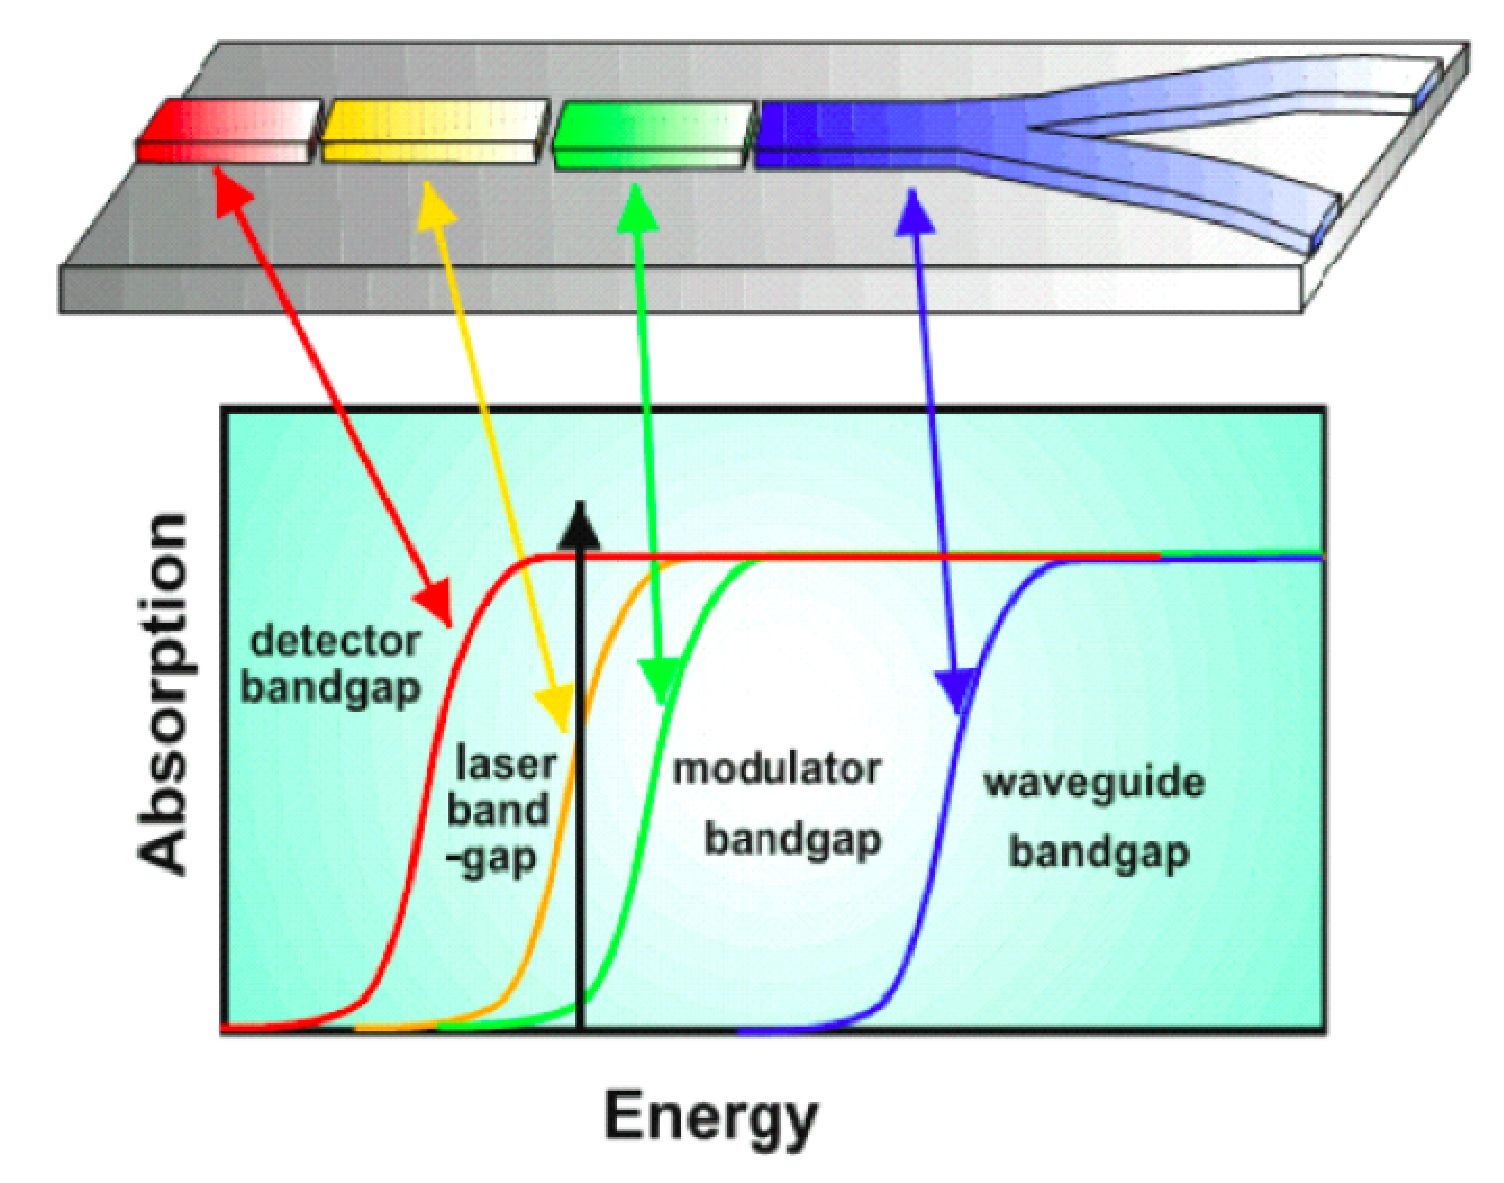
\includegraphics[width=0.7\textwidth]{./Pictures/pic.eps}\\
  \caption{光子集成回路示意图}
  \label{fig_pic}
\end{figure}

总的来说,任何一种单片集成的方法至少需要达到以下几条要求:

\begin{enumerate}
\item{精确的改变每个分立器件的材料的禁带宽度}
\item{空间分辨率应该远小于器件的尺寸}
\item{材料的其他特性应该尽量保持不变,比如折射率、损耗、电特性等}
\end{enumerate}

\section{单片集成技术的方法}

为了在一块芯片上做出不同的禁带宽度,在过去的几十年中,已经有很多种方法实现这样的效果。然而,每一种方法都有他的优点和缺点,所以在实际生产中,还没有形成一种通常的解决方案,这也是该领域值得研究的一个问题。图\ref{fig_pic_methods}例举了几十年来人们所研究的各种单片集成方法。

\begin{figure}[!htb]
  \centering
  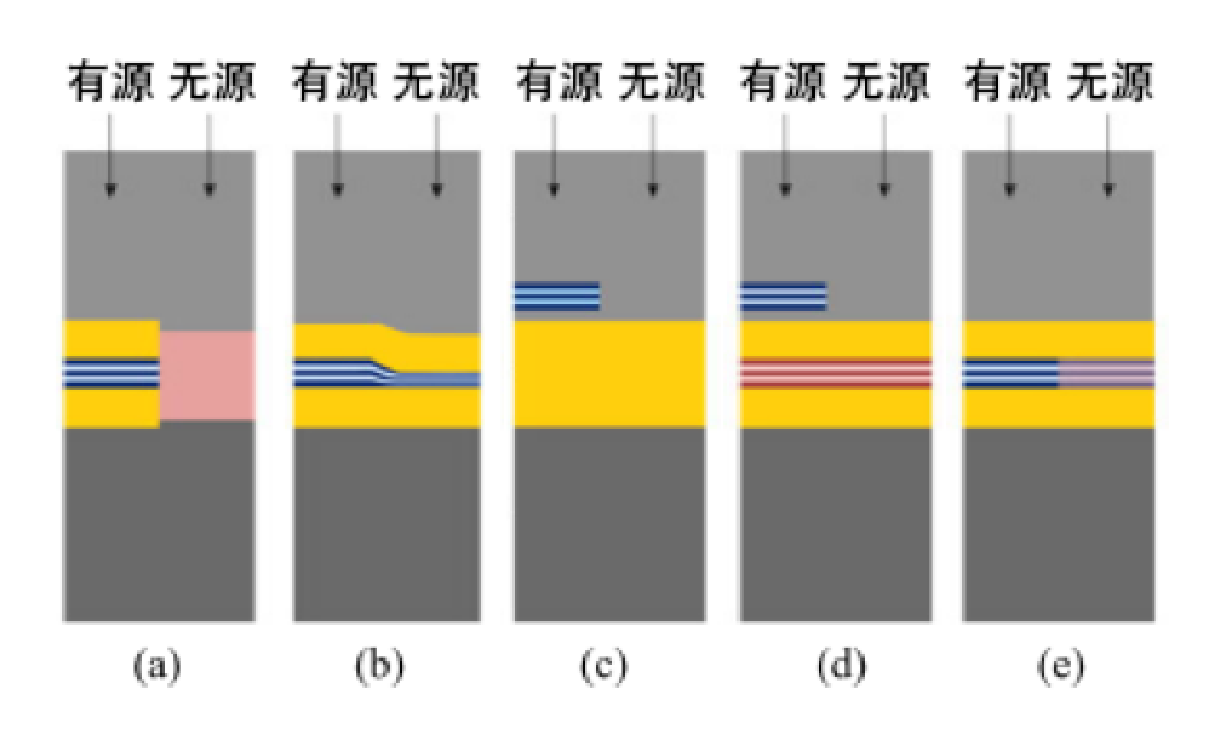
\includegraphics[width=0.7\textwidth]{./Pictures/pic_methods.eps}\\
  \caption{有源和无源器件单片集成的各种方法}
  \label{fig_pic_methods}
\end{figure}

\subsection{对接再生长}

对接再生长的方法如图\ref{fig_pic_methods}的第1种方法所示。这种方法的原理是,首先生长一片全部包含有源层的芯片,然后将无源部分的芯层刻蚀掉,最后在这些地方重新生长无源的芯层和包层。这种方法的优点是,每个部分的材料禁带宽度都可以非常准确的控制。同时,它的缺点也是显而易见的。由于有源的芯层和无源的芯层必须对准,而通常的量子阱片芯层仅有几十纳米,所以这给工艺带来了不小的难度。此外,如果需要制作多种不同禁带宽度的材料,就需要进行多次的刻蚀和再生长,大大增加了工艺的复杂度。最后,由于之后生长上去的材料和原先的材料完全不同,所以很可能存在较大的折射率差,这样会导致界面上的光被反射,增加了额外的损耗。近年来,很多人通过改进工艺,大大减小了界面的反射率,这个问题已经不再是一个问题。总而言之,这种方法最直接、最有效,同时在工艺上的难度和复杂度限制了它的发展。

\subsection{选择性区域生长}

选择性区域生长的方法如图\ref{fig_pic_methods}的第2种方法所示。这种方法只需要一步生长就可以完成,所以是对对接再生长的改进。这种方法的原理是,在芯片生长芯层之前,先在芯片上生长一层介质膜。然后,在用金属氧化物化学气相沉积(MOCVD)生长芯层的过程中,由于介质膜的影响,材料的厚度和组分会发生变化,导致禁带宽度的改变。只要介质膜生长得当,这种方法可以一次性生长出多个需要的禁带宽度的材料。不过,这种方法对MOCVD生长条件的控制非常苛刻,所以工艺难度非常高。

\subsection{偏置量子阱}

图\ref{fig_pic_methods}的第3种方法是偏置量子阱方法。这种方法的原理是,有源层的芯层被生长在无源层的芯层之上,最后在无源区域刻蚀掉有源层的芯层。这种方法比较简单直接,但是缺点似乎更多。首先,它只能将两种禁带宽度的材料集成在一起。然后,由于有源芯层不在最中间,激光器的限制因子会大大下降,这样会大大减小激光器的增益。最后,无源部分不包含量子阱层,所以在制作调制器时,性能会大打折扣。

\subsection{双量子阱}

图\ref{fig_pic_methods}的第4种方法是双量子阱方法。显然,该方法是偏置量子阱方法的改进。它在偏置量子阱的基础上,在无源芯层也生长了量子阱。这样可以解决调制器的性能问题。可是这种方法并不能解决偏置量子阱方法的其他问题,例如激光器限制因子仍然比较低等等。

\subsection{量子阱混杂技术}

从制作工艺的角度来说,图\ref{fig_pic_methods}的第5种方法所示的量子阱混杂技术可能是最简单的单片集成方法。如图\ref{fig_qwi}所示,对于普通的量子阱材料来说,沿着材料的生长方向看过去,每一层材料的禁带宽度是一种矩形的结构。整个量子阱的禁带宽度是由阱的材料和厚度,以及垒的材料决定的。然后,当我们通过某种方法,将阱和垒的材料进行融合,使量子阱的每一层的禁带宽度变成一个渐变的结构之后,整个材料的禁带宽度就会发生变化(通常是禁带宽度增加)。所以,我们只需要在芯片生长完之后,制作各个部分的器件之前,对调制器和无源波导区域进行量子阱混杂,其中禁带宽度的增加量由混杂的工艺参数决定,这样就可以实线单片集成的效果。

\begin{figure}[!htb]
  \centering
  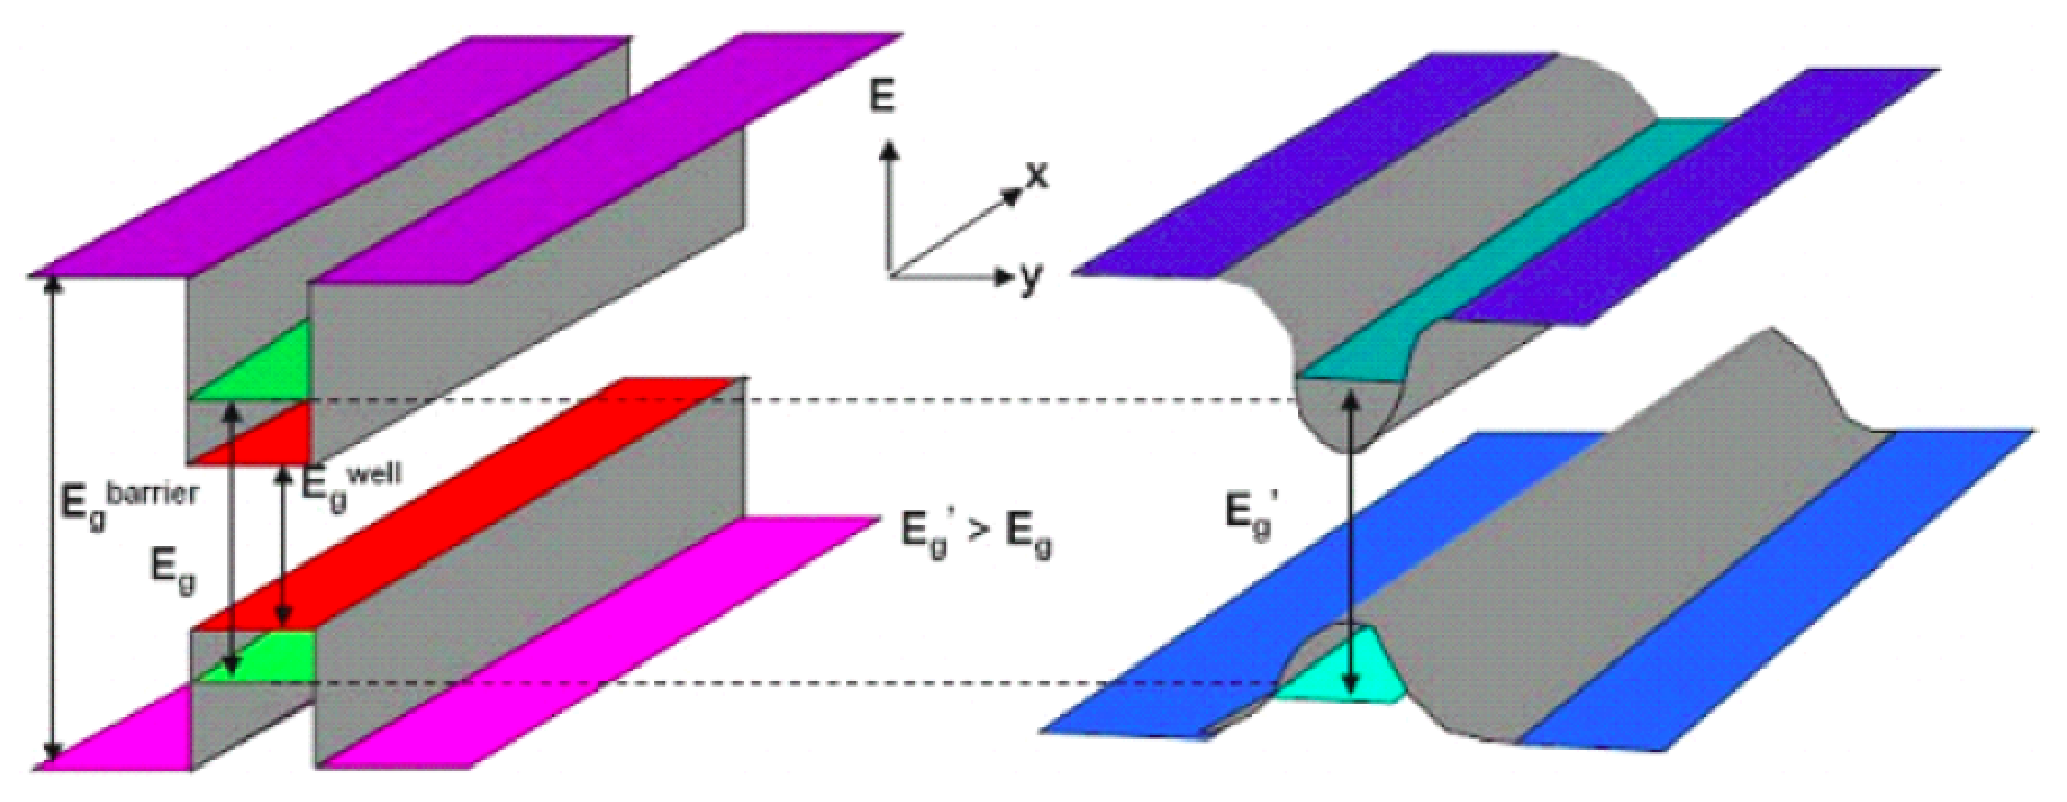
\includegraphics[width=0.7\textwidth]{./Pictures/qwi.eps}\\
  \caption{量子阱混杂技术示意图}
  \label{fig_qwi}
\end{figure}

然而,只通过一般的退火的方法是不可能达到量子阱混杂的效果的。因为量子阱是十分稳定的,只有在非常高的温度和非常长的时间作用下,才会开始发生混杂现象(此处需要补充一篇文献)。为了让混杂在较低的温度和较短的时间内发生,通常会在芯片的表面或者内部产生一些缺陷。这些缺陷在快速退火的条件下,可以快速扩散到量子阱层,引起阱和垒互相扩散,达到量子阱混杂的目的。

\subsection{各种单片集成技术的比较}

\section{量子阱混杂技术回顾}

量子阱混杂是一个量子阱的阱和垒相互扩散的过程。在这个过程中,随着扩散的不断增强,量子阱的形状和厚度也随之不断变化,从而导致能带的变化。变化之后的能带对应的能量一般来说都是增加的,也就是波长发生蓝移。在一般情况下,量子阱的阱和势垒之间的界面是亚稳态的,在一定的条件下,例如高温下,量子阱的阱和势垒的原子会相互扩散。量子阱混杂的目标不是简单地使阱和势垒相互扩散,而是在整个区域中做选择性的扩散。

已经有很多种方法可以实现量子阱混杂的效果,例如杂质诱导无序(IID) \cite{holonyak1998impurity-IID} ,无杂质空位增强无序(IFVD) \cite{si1998area-IFVD},光吸收诱导无序(PAID) \cite{mckee1997monolithic-PAID},离子注入增强扩散\cite{charbonneau1998photonic-implantation}等等。本节将介绍最近几十年中研究过的绝大部分方法,并进行比较。

\subsection{杂质诱导方法}

\begin{figure}[!htb]
  \centering
  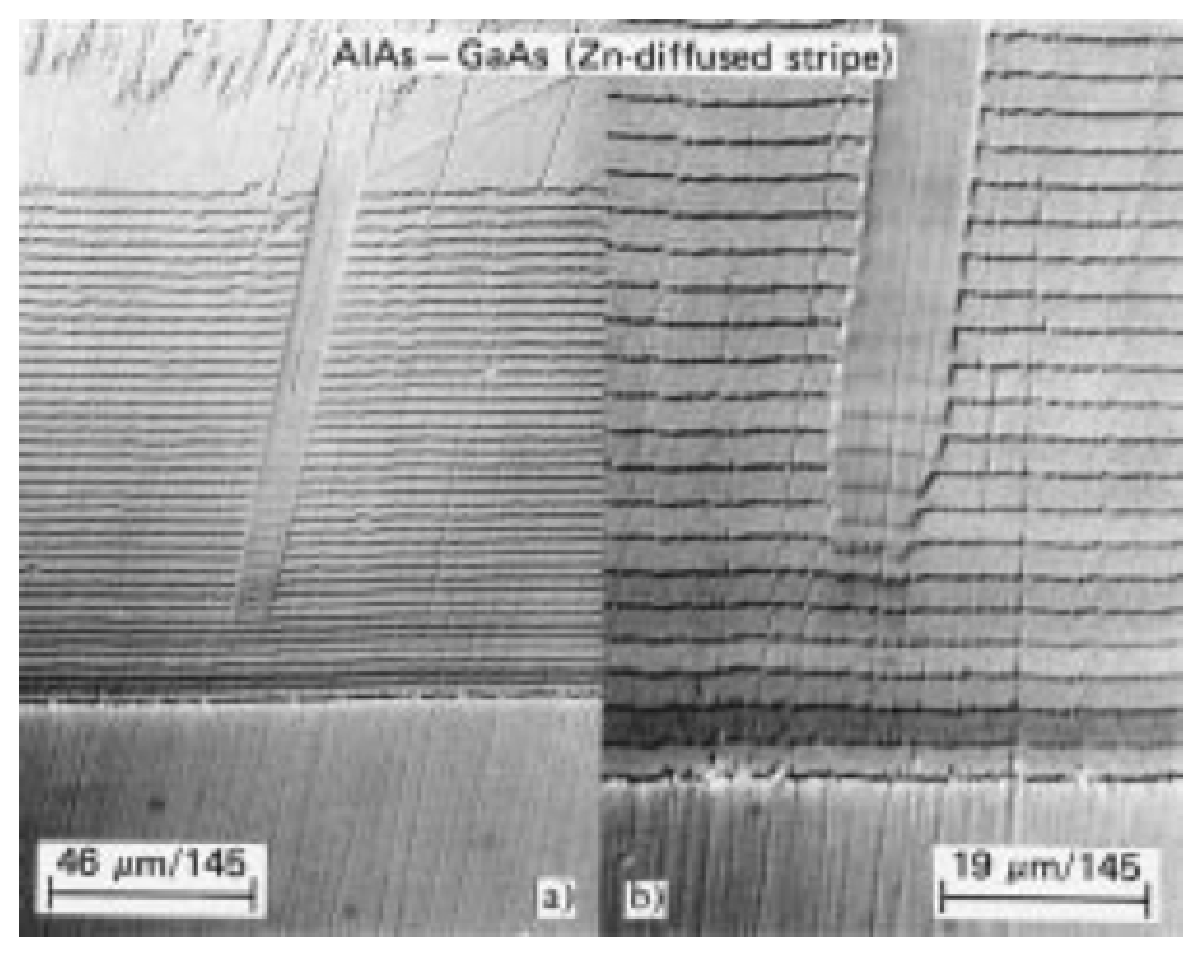
\includegraphics[width=0.7\textwidth]{./Pictures/iid.eps}\\
  \caption{Zn扩散到AlAs-GaAs超晶格中引起混杂的电镜图片}
  \label{fig_iid}
\end{figure}

19世纪80年代,人们开始研究量子阱混杂技术,第一个被想到和实现的是杂志诱导方法。1981年,美国伊利诺斯大学的W. D. Laidig等人提出了使用Zn扩散到AlAs-GaAs超晶格中引起混杂的方法\cite{laidig1981disorder},这也是第一次报道的杂质诱导方法(更详细的介绍可以参考一份相关的专利\cite{holonyak1983method})。如图\ref{fig_iid}所示,在AlAs-GaAs超晶格的中间10um区域,已经有Zn原子扩散到里面,扩散的温度仅仅需要575摄氏度,大大低于GaAs材料本身发生混杂的温度。在Zn扩散进去之后,AlAs-GaAs超晶格的组分发生了变化,变成了AlGaAs的三元合金,材料的禁带宽度也随之增加了。在这个实验中,为了达到Zn原子选择性扩散的目的,芯片表面利用光刻技术覆盖了一层Si3N4掩膜,然后和ZnAs2一起放入专门的扩散炉中,在500-600摄氏度的条件下等待10-60分钟,就可以在没有覆盖Si3N4的地方达到混杂的效果。

此后,人们在这篇文章的基础上,对杂质诱导方法进行了大量研究和改进。例如,美国罗克韦尔国际微电子研究发展中心的J. J. Coleman等人提出了用低能的Si离子注入实现AlAs-GaAs超晶格混杂的方法\cite{coleman1982disorder}。他们使用375keV能量的Si离子,注入到AlAs-GaAs超晶格芯片的表面,然后在退火的作用下,达到了混杂的目的。此后,人们发现了Ge,S,Sn,Se,Be,Mg等原子也可以达到杂质诱导混杂的目的(此处可以添加5-9篇文章)。1984年,美国麻省理工学院在InGaAsP量子阱材料上也实现了杂质诱导混杂的效果。他们用这种方法制作了10GHz的激光器和调制器集成的器件\cite{tsang1981intracavity}。

(此处应添加其缺点,不过暂时没看出来)

\subsection{无杂质空位诱导方法}

\subsection{阳极氧化诱导方法}

1998年,香港大学的Shu Yuan等人提出了一种在GaAs量子阱芯片上采用阳极氧化实现量子阱混杂的方法\cite{yuan1998anodic}\cite{yuan1998anodicJSTQE}。其工艺设备如图\ref{fig_oxide}所示。首先,GaAs量子阱片被固定在一个开路的50伏脉冲式电源的阳极上。阳极和阴极之间通过导电液传到电流。导电液由乙二醇、磷酸和去离子水用40:20:1的体积比配制而成。芯片的一半由导热胶覆盖,这样一来,只有另一半暴露在导电液中的部分会被氧化。经过几分钟的脉冲电流处理之后,芯片又进行了快速退火处理。最终的测试结果如图\ref{fig_oxide_pl}所示。在芯片没有被氧化的部分,光致发光谱的峰值波长仅仅蓝移了5meV左右,同时强度下降到只剩原来的1/20。而对于氧化过的部分,蓝移达到了44meV,而强度上升到了原来的两倍多。可见,这种方法在获得较大蓝移的同时,还可以增加光致发光谱的强度。

\begin{figure}[!htb]
  \centering
  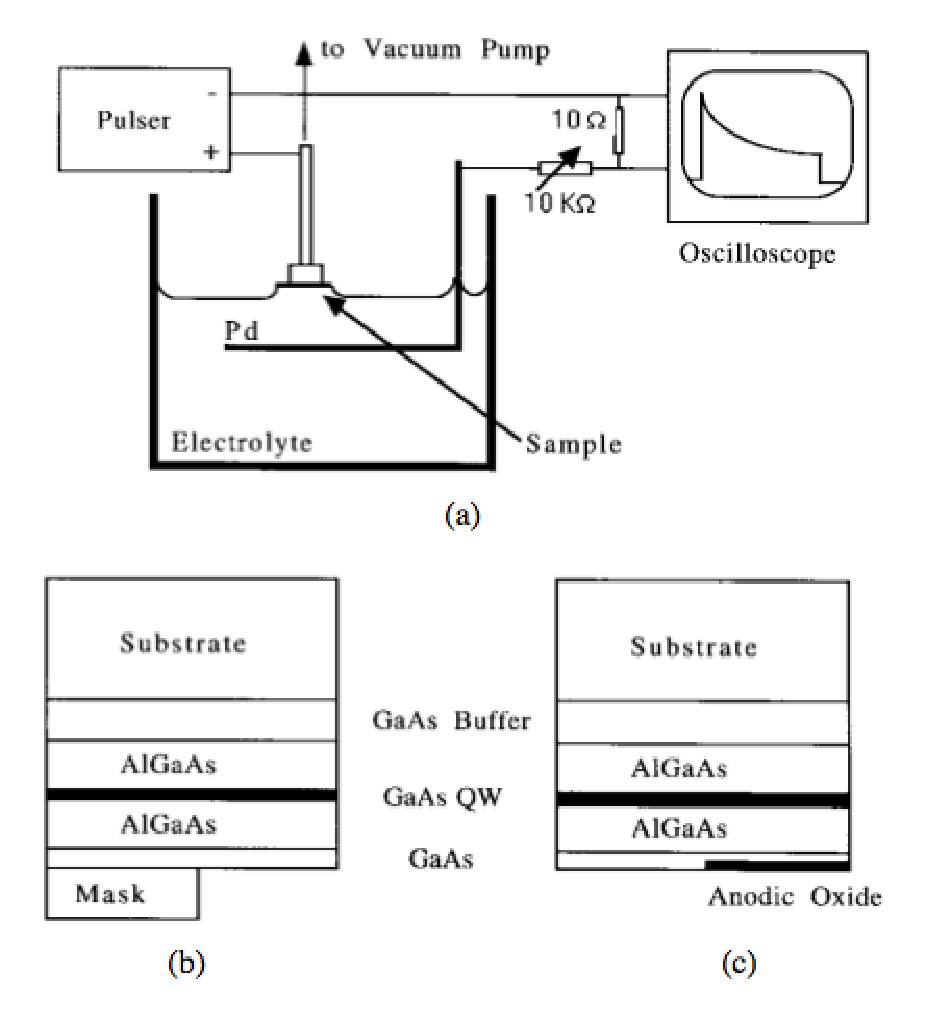
\includegraphics[width=0.7\textwidth]{./Pictures/oxide.eps}\\
  \caption{阳极氧化诱导量子阱混杂技术的设备示意图}
  \label{fig_oxide}
\end{figure}

\begin{figure}[!htb]
  \centering
  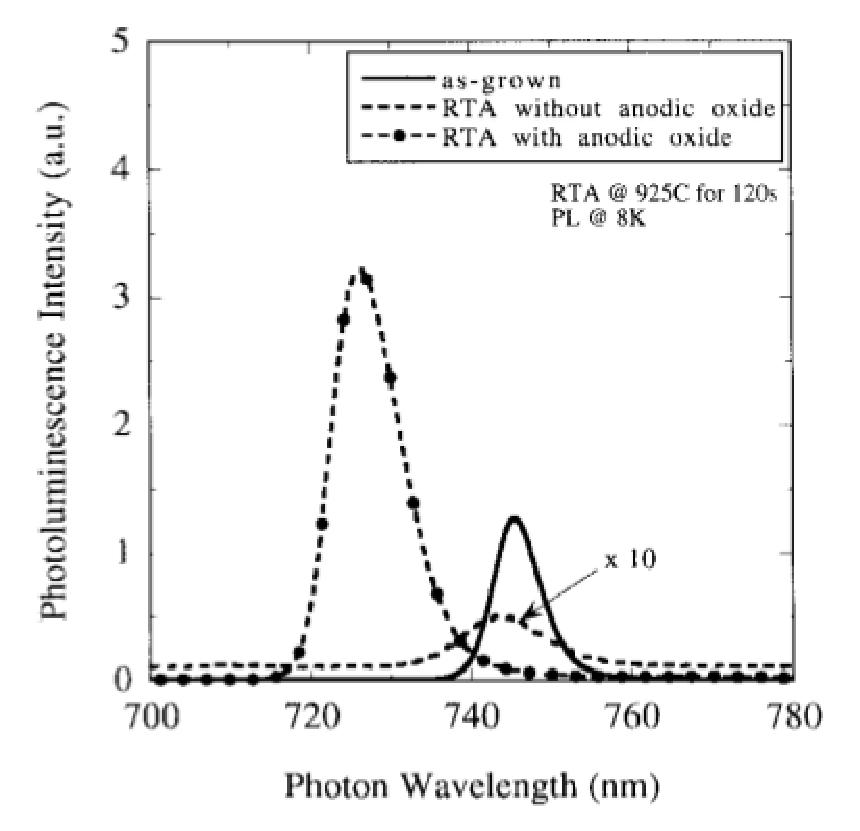
\includegraphics[width=0.7\textwidth]{./Pictures/oxide_pl.eps}\\
  \caption{混杂前后的光致发光谱测试结果}
  \label{fig_oxide_pl}
\end{figure}

可惜的是,这种方法由于需要非常特殊的实验条件,后来并没有进行广泛研究。这种方法也只能停留在研究光致发光谱蓝移的方向上,并没有应用到任何器件上,也没有在InP量子阱材料上成功实现。尽管如此,人们一直没有忘记这种方法,因为氧化与其他很多方法在原理上不谋而合\cite{dubowski1999enhanced}\cite{liu2012xps}\cite{liu2013chemical}。

\subsection{光吸收诱导方法}

1997年,英国格拉斯哥大学的Andrew McKee等人提出了用激光照射实现量子阱混杂的方法\cite{mckee1997monolithic-PAID}。该方法使用Nd:YAG激光器照射芯片的表面。由于Nd:YAG激光器发出的光波长在1064nm左右,介于InP的波长和芯层1550nm波长之间,所以正好可以穿过InP包层直接被芯层吸收,达到类似于加热退火的作用。整个工艺的过程是这样的。首先,芯片的表面会生长一层500nm厚的二氧化硅,既可以作为减反射薄膜,又可以对芯片表面原子起到一定的保护作用。然后,芯片被放在200摄氏度的热盘上,这样既可以提供一个背景温度,减小了Nd:YAG激光器照射所需的能量,又可以防止加热后的芯片过快地将热量往下散发。最后,Nd:YAG激光器输出$5W/mm^2$的光,照射芯片30分钟。该方法可以得到最大160nm的蓝移,这是相当可观的,同时还能保持材料的优良性能。混杂之后的激光器,计算得到的损耗甚至比混杂之前的还要小,这说明该方法不会增加甚至减小材料的损耗。由这种方法制作的无源波导,损耗仅有$5dB/cm$。

虽然这种方法效果很好,但是这种方法的致命缺陷在于,长时间的照射会让空间分辨率变得很差。2004年,美国利哈伊大学的Boon Siew Ooi等人提出了采用脉冲光吸收的新方法\cite{ooi2004multiple}。该方法采用一个Q调制的Nd:YAG激光器(10Hz,2.8-3.9$mJ/mm^2$,1-10分钟)照射芯片,然后再进行快速退火(625摄氏度,120秒)的方法。显然这种方法与采用连续Nd:YAG激光器照射的方法相比,原理是不同的。虽然波长一样,但是它产生的光只能被芯片表层的InGaAs吸收,并且在它的表面产生缺陷。这层缺陷在之后的快速退火中往下扩散,达到混杂的目的。这种方法制作的芯片除了有连续激光器照射方法的优点之外,其空间分辨率达到了2.5um,完全达到了单片集成的要求。

\subsection{等离子体轰击方法}

2002年,新加坡南阳理工大学的Ting Mei教授团队提出了用等离子体刻蚀机和快速退火的实现量子阱混杂的方法\cite{djie2002high}。该方法首先利用等离子体刻蚀机形成的氩气等离子体轰击芯片的表面,形成一层非常薄(约10nm)的缺陷层。然后,在快速退火的作用下,这层缺陷往下扩散到量子阱层,促进量子阱的阱和垒的互相融合,达到量子阱混杂的目的。与其他的方法相比,这种方法最大的优点在于,我们不需要为了量子阱混杂购买额外的设备,因为等离子体刻蚀机是刻蚀芯片必须的设备,而快速退火也会在制作电极的欧姆接触时用到。而且,其工艺步骤非常简单,只需要等离子体轰击和快速退火两步就可以完成。如果需要对芯片做选择性的量子阱混杂,只需要在不做混杂的区域覆盖一层光刻胶或者二氧化硅掩膜,用来阻挡氩气等离子体的轰击就可以实现。2005年,该团队报道了利用这个方法制作的延长腔激光器\cite{djie2005plasma},也是至今为止唯一报道的用等离子体轰击方法制作的有源和无源单片集成的器件。很有意思的是,他们还发现了芯片表面的掺杂情况会对量子阱混杂的效果产生很大影响\cite{xu2009inductively}。

虽然这种方法具有工艺简单,成本低,效果好等优点,并且已经有了延长腔激光器这样的简单的集成应用,但是人们发现它的可重复性存在很大的问题。2011年,浙江大学的彭盛华硕士重复了上面的实验\cite{peng2011argon},其中所用的等离子体刻蚀机与南阳理工大学的刻蚀机是同一型号的(Oxford ICP 100)。在类似的工艺参数条件下他们发现,尽管材料的禁带宽度也可以蓝移100nm以上,但是光致发光谱的强度下降了一半左右。当他们把氩气等离子体换成氮气之后,同样发现光致发光谱下降了很多\cite{peng2009nitrogen-nitrogen}。用这种方法制作的无源波导测试得到的损耗达到了$68dB/cm$\cite{zhang2010optical-waveguide_test},完全达不到无缘器件集成的要求。所以,这种方法只有在蓝移50nm左右的情况下可以做得较好。或者在没有上包层的芯片上做,然后再生长上包层,这样又大大增加了工艺的复杂度。总的来说,用等离子体轰击方法实现量子阱混杂的方法还有待进一步的研究。

\subsection{溅射轰击方法}

溅射轰击方法与等离子体轰击方法的原理非常相似。首先,芯片在溅射的过程中,在表面产生一层很薄的缺陷层。然后,这层缺陷在快速退火的条件下快速运动到量子阱区域,促进阱和垒的互相扩散,达到量子阱混杂的目的。这种方法也不需要购买额外的设备,因为溅射机是制作激光器电极的设备。如果需要对芯片做选择性的量子阱混杂,只需要在不做混杂的区域覆盖一层光刻胶或者二氧化硅掩膜,这些特点与等离子体轰击方法完全相同。不同的地方在于溅射的靶的材料。1998年,英国格拉斯哥大学的John Marsh教授团队提出了利用溅射二氧化硅和快速退火的方法实现量子阱混杂的效果\cite{mcdougall1998monolithic}。2014年,浙江大学的朱宏力博士提出了溅射氧化铝\cite{zhu2014quantum}和氮化硅\cite{zhu2014bandgap}实现量子阱混杂的技术。

\subsection{离子注入方法}

离子注入方法由离子注入和快速退火两个步骤组成。首先,特定种类的离子在非常高能量的离子注入机的加速下,直接打入芯片的内部。然后,在快速退火的作用下,这些离子促进了量子阱中的阱和垒的融合,最终达到改变禁带宽度的目的。

\begin{figure}[!htb]
  \centering
  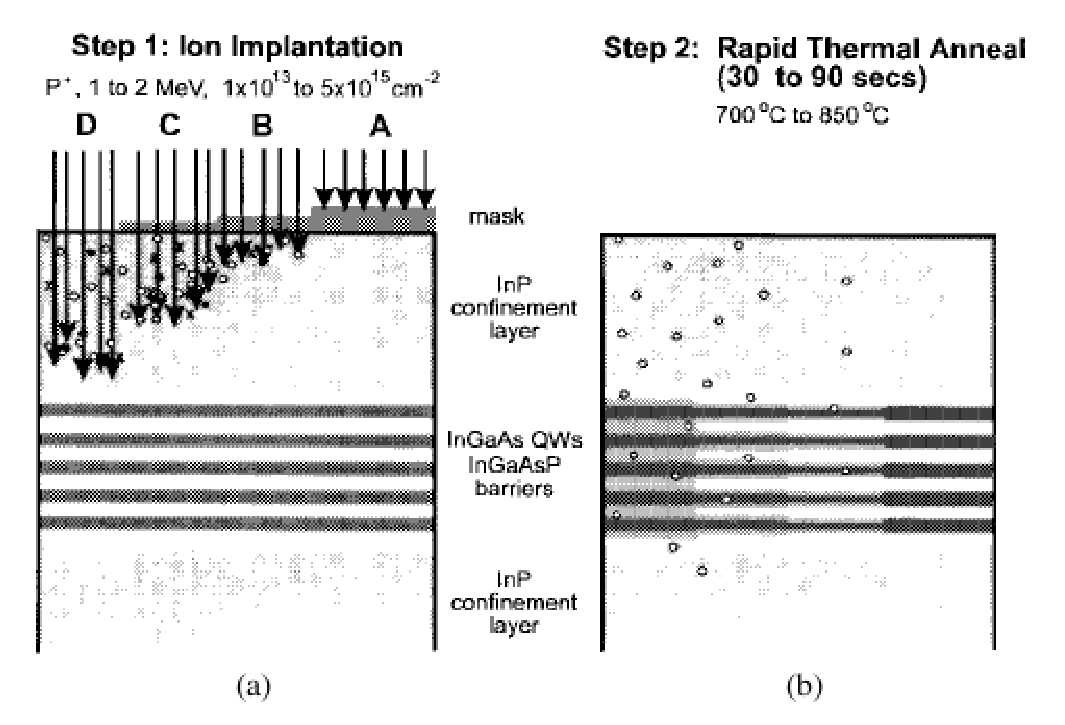
\includegraphics[width=0.7\textwidth]{./Pictures/implantation.eps}\\
  \caption{离子注入技术示意图}
  \label{fig_implantation}
\end{figure}

如图\ref{fig_implantation}所示,在D区域,磷离子在离子注入机的加速下直接注入到芯片的上包层,并在之后的快速退火的作用下,促进量子阱的阱和垒的互相融合。最有意思的是,在C、B、A区域,芯片表面生长了一层$SiO_2$掩膜。这层掩膜可以抵消一部分离子注入的能量,导致离子只能注入到稍浅的地方,最终这些区域的量子阱混杂程度会比没有掩膜的地方稍弱。通过制作不同厚度的$SiO_2$掩膜,就可以精确地控制量子阱混杂的程度,并且只需要一次快速退火就可以形成很多个不同禁带宽度的区域。

离子注入方法制作的无源波导的性能甚至比量子阱混杂之前的性能还要好。如图\ref{fig_implantation_wg_test}所示,量子阱混杂之后,波导的禁带宽度相比于未混杂的波导,蓝移了90nm左右。计算得到的损耗如图\ref{fig_implantation_wg_loss}所示。对于未混杂的波导,在透明传输的波长区域,比如1580nm,波导的损耗大约是$8cm^{-1}$。对应到混杂之后的波导的1490nm,波导的损耗只有$5cm^{-1}$左右。也就是说,经过离子注入方法制作的无源波导,损耗可以比未做处理之前还要低。

\begin{figure}[!htb]
  \centering
  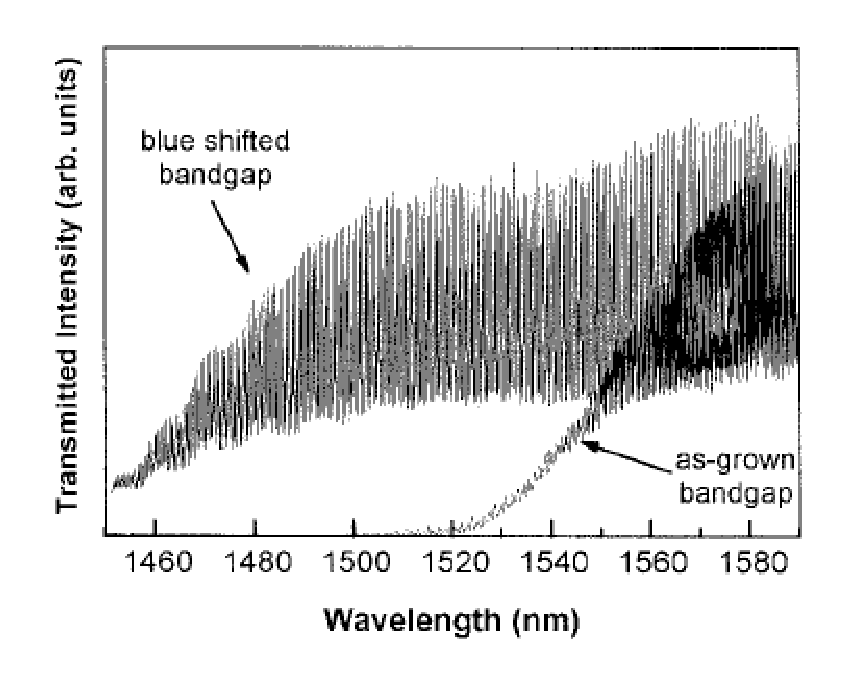
\includegraphics[width=0.7\textwidth]{./Pictures/implantation_wg_test.eps}\\
  \caption{测试得到的量子阱混杂和未混杂波导的透射光谱}
  \label{fig_implantation_wg_test}
\end{figure}

\begin{figure}[!htb]
  \centering
  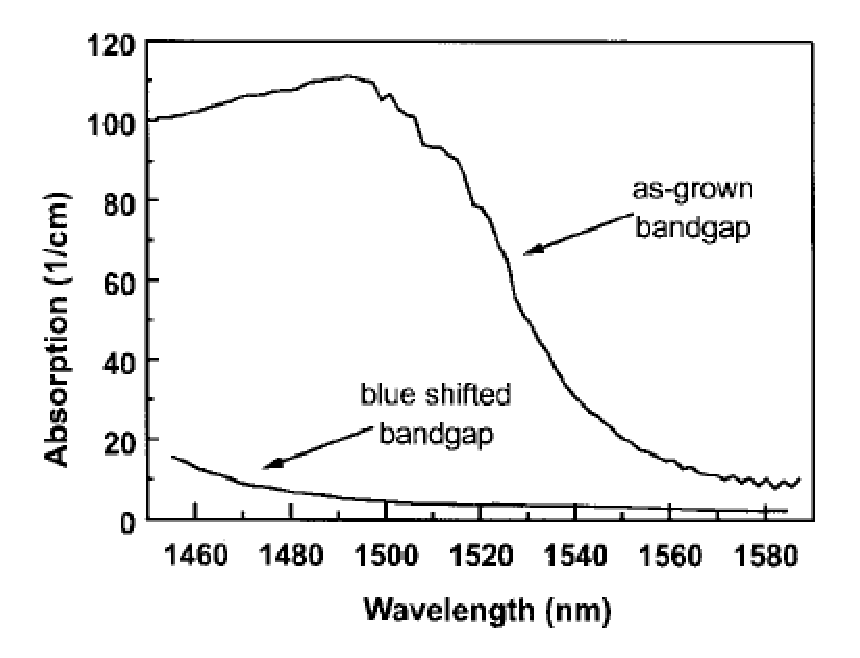
\includegraphics[width=0.7\textwidth]{./Pictures/implantation_wg_loss.eps}\\
  \caption{由透射光谱计算得到的损耗}
  \label{fig_implantation_wg_loss}
\end{figure}

利用离子注入技术制作的激光器的IV特性曲线如图\ref{fig_implantation_laser}所示。从图中可以看出,在量子阱混杂前后,两种激光器的IV曲线是非常相似的。在激光器工作的第一象限,两条曲线基本重合在一起。这说明,离子注入技术不会改变材料的电特性。

\begin{figure}[!htb]
  \centering
  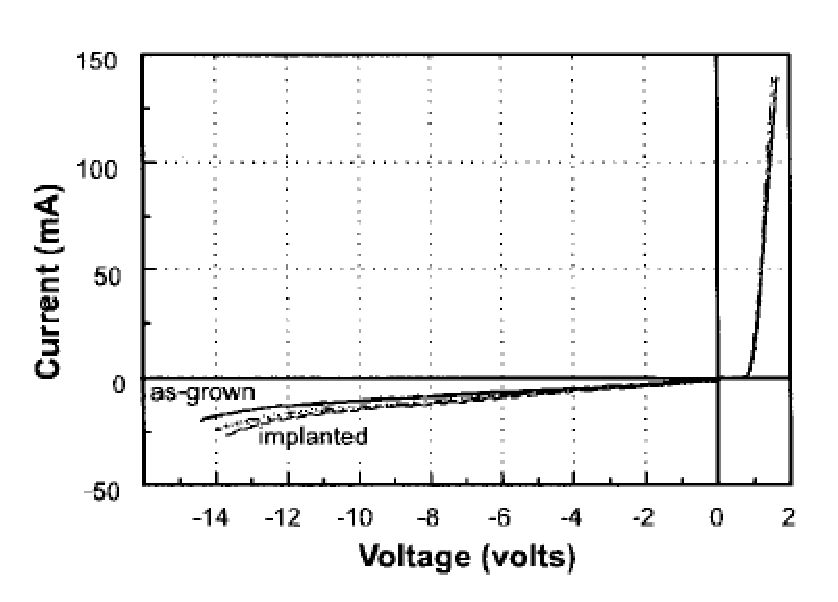
\includegraphics[width=0.7\textwidth]{./Pictures/implantation_laser.eps}\\
  \caption{由离子注入方法制作的激光器的IV特性曲线}
  \label{fig_implantation_laser}
\end{figure}

由于离子注入技术相对成熟,性能也很好,人们已经利用该技术制作了非常复杂的单片集成器件。加州大学圣巴巴拉校区的Larry Coldren教授团队报道了一个$8\times8$InP单片集成波长可调路由器\cite{nicholes20108},也是当时世界上最复杂的单片集成光器件,实物图如图\ref{fig_motor}所示。该器件需要集成8个取样光栅分布式布拉格反射激光器(SGDBR),8个波长转换器以及1个阵列波导光栅等器件。因为所有的器件都需要对部分或全部的区域进行量子阱混杂处理,在每个器件制作之前,芯片的大部分区域都采用了离子注入技术进行处理,材料的禁带宽度从原先的1545nm蓝移到了1420nm。

\begin{figure}[!htb]
  \centering
  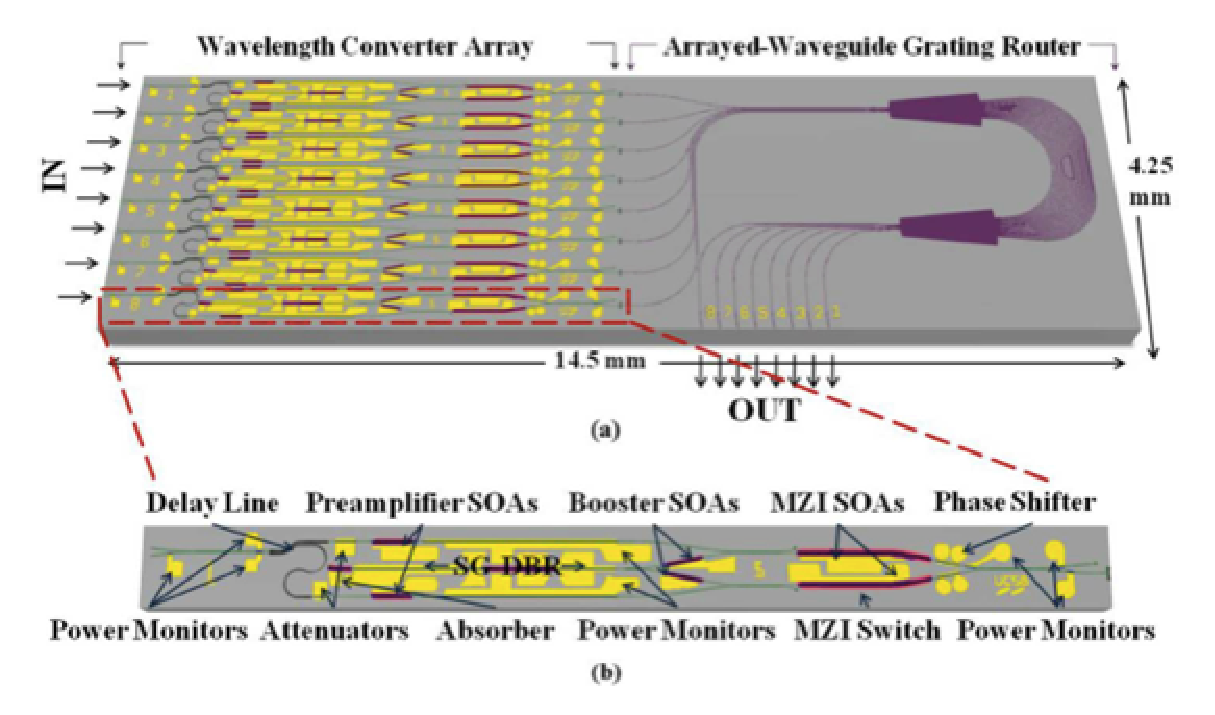
\includegraphics[width=0.7\textwidth]{./Pictures/motor.eps}\\
  \caption{$8\times8$InP单片集成波长可调路由器}
  \label{fig_motor}
\end{figure}

\subsection{各种量子阱混杂方法的比较}

%%%%%%%%%%%%%%%%%
\chapter{量子阱混杂技术的理论模拟}

在量子阱混杂工艺研究不断取得进展的同时,人们也做了很多量子阱混杂的理论模拟方面的工作。这些模拟让人们更好地理解了量子阱混杂的机理,并指导人们在工艺上进一步优化。量子阱混杂的理论模拟最核心的问题是计算混杂之后的能带结构。也就是说,在原有的量子阱的基础上,通过加入混杂的工艺参数作为变量,计算得到混杂之后的能带结构。有了能带结构之后,就可以进一步计算材料的吸收系数,增益,折射率等等。最后,就可以计算出量子阱混杂对整个光器件的影响。这一章将详细介绍量子阱混杂的能带结构的计算方法。

\section{量子阱能带计算}

在半导体中,电子运动的状态可以通过解薛定谔方程得到。

\begin{equation}
    \label{schrodinger}
    \frac{-h^2}{2} \frac{d}{dz} \frac{1}{m_\perp^*(z)} \frac{d\varphi(z)}{dz}
    +V(z)\varphi(z)
        = E\varphi(z)
\end{equation}

其中,$m_\perp(z)$是导带或者价带的有效质量。$V(z)$是导带或者价带的势函数。(需要结合量子力学的课本重写)

然后,我们采用包络函数近似(?)对上面的方程进行简化。在这个近似中,波函数的时间和空间分量可以分离开来,得到如下的函数式

其中??是波函数的稳态解,E是能量特征值。接着,我们还需要用有效质量近似(?)再对薛定谔方程做一次简化,并且写成一维方向上的函数式,最后可以写成

\begin{equation}
    \label{eq_effective_mass}
    \left[ \frac{-\hbar^2}{2} \frac{d}{dx} \frac{1}{m^*(x)} + V(x) \right] \psi(x) = E \psi(x)
\end{equation}

我们只需要知道有效质量$m^*(x)$和势能$V(x)$在每个x上的值,就可以求出整个系统的特征值和特征函数,对应半导体能级的能量$E$和波函数$\psi(x)$。求解上述方程的数值方法有很多,包括有限差分法、传输矩阵法和有限元法等等。我们选择了相对简单,并且精度足够用的传输矩阵法。首先,我们需要将上面方程中的势函数和有效质量进行离散化,如图\ref{fig_tmm}所示。在每一小段的离散区间内,势函数和有效质量被视为不变,也就是说,在$x_j\le x<x_j+\Delta_j=x_{j+1}$时,$V_j=V(x_j)$,$m^*_j=m^*(x_j)$,而在这一段的末尾进行$V_j\to V_{j+1}$,$m^*_j\to m^*_{j+1}$的跳变。在$x_j\le x<x_{j+1}$的区间内,方程\ref{eq_effective_mass}的解可以表示为

\begin{equation}
    \label{eq_effective_mass_solution}
    \psi(x) = A_j \exp [i k_j (x-x_j)] + B_j \exp [-i k_j (x-x_j)]
\end{equation}

\begin{figure}[!htb]
  \centering
  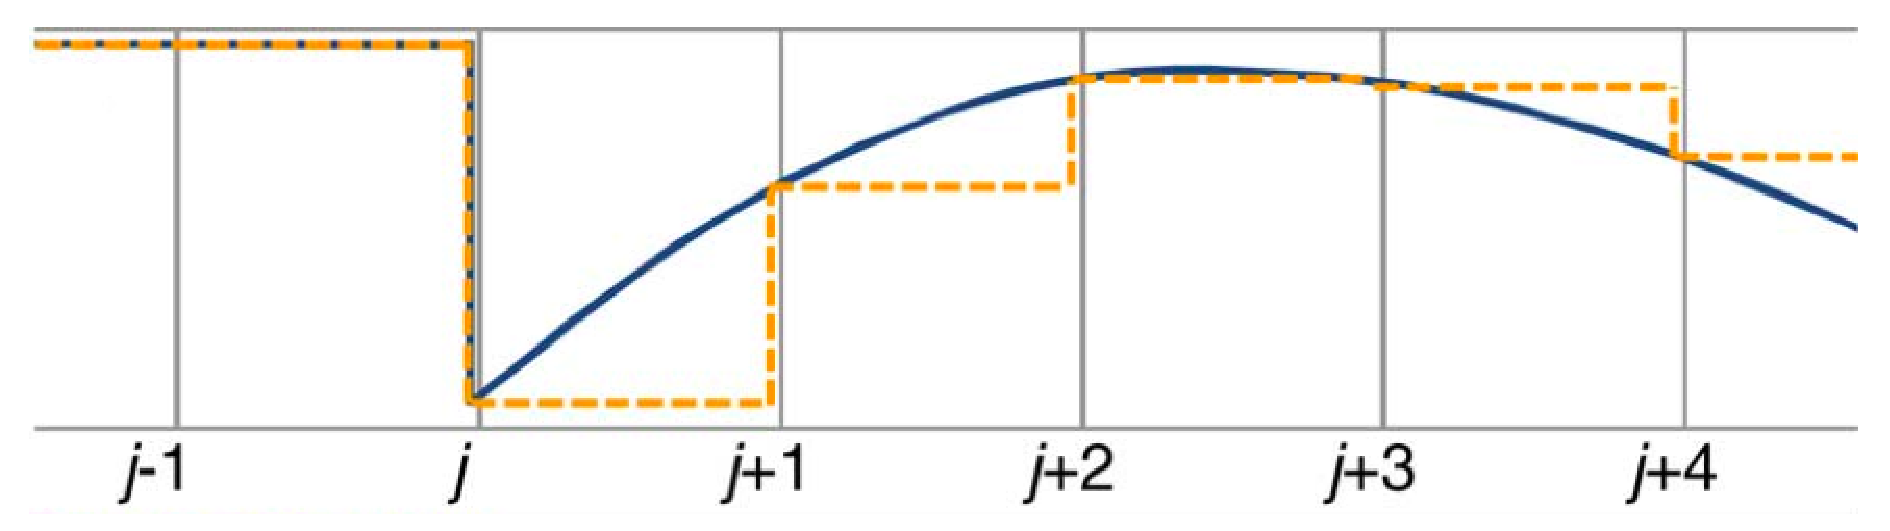
\includegraphics[width=0.7\textwidth]{./Pictures/tmm.eps}\\
  \caption{传输矩阵法对势函数和有效质量的离散化,实线代表精确值,虚线代表离散值}
  \label{fig_tmm}
\end{figure}

其中$k_j=\sqrt{2 m^*_j (E-V_j)} / \hbar$是波函数的波数。同时,方程\ref{eq_effective_mass}的边界条件需要满足波函数和它的导数在每个区间的连接点上连续,即如下两个方程

\begin{equation}
    \label{eq_boundary_1}
    \psi_{j-1}(x_{j-1}) = \psi_j(x_{j-1}) 
\end{equation}

\begin{equation}
    \label{eq_boundary_2}
    \frac{1}{m^*_{j-1}} \frac{d}{dx} [ \psi_{j-1}(x_{j-1}) ] = \frac{1}{m^*_j} \frac{d}{dx} [\psi_j(x_{j-1})]
\end{equation}

将边界条件方程\ref{eq_boundary_1}和\ref{eq_boundary_2}代入方程\ref{eq_effective_mass},就可以得到相邻两层的波函数振幅之间的关系,即

\begin{equation}
    \label{eq_tmm}
    \begin{pmatrix} A_{j+1} \\ B_{j+1} \end{pmatrix} = T_{j,j+1} \begin{pmatrix} A_{j} \\ B_{j} \end{pmatrix}
\end{equation}

其中的传输矩阵为

\begin{equation}
    \label{eq_transfer_matrix}
    T_{j,j+1} = \frac{1}{2\beta_{j+1}} \begin{pmatrix} \beta_{j+1}+\beta_j & \beta_{j+1}-\beta_j  \\ \beta_{j+1}-\beta_j  & \beta_{j+1}+\beta_j  \end{pmatrix} \begin{pmatrix} e^{ik_j\Delta_j} & 0 \\ 0 & e^{-ik_j\Delta_j} \end{pmatrix}
\end{equation}

其中$\beta_j = k_j/m^*_j$。最后,我们可以将每一层的传输矩阵从左往右连续相乘,得到如下的方程

\begin{equation}
    \label{eq_tmm_serial}
    \begin{pmatrix} A_{N} \\ B_{N} \end{pmatrix} = T_{N-1,N}T_{N-2,N-1}\cdots T_{0,1} \begin{pmatrix} A_{0} \\ B_{0} \end{pmatrix} =  \begin{pmatrix} T_{11} & T_{12} \\ T_{21} & T_{22} \end{pmatrix} \begin{pmatrix} A_{0} \\ B_{0} \end{pmatrix}
\end{equation}

其中$N$是分段的总段数。这个连续的方程需要满足收敛条件,也就是$A_0=B_N=0$,对应于最后的方程

\begin{equation}
    \label{eq_t22}
    T_{22}=0
\end{equation}

上面的方程是一个关于E的复数方程,它的所有解,从小到大依次就是每一个能级,代入到前面的波动方程\ref{eq_effective_mass_solution}中,就可以得到每个x点上的波函数。

为了验证程序的正确性,我们选择了文献中的AlGaAs-GaAs量子阱结构\cite{jonsson1990solving},其势能和有效质量如表\ref{tmm_sample}所示。由于导带和价带的能级计算方法完全一样,这里只给出导带的计算结果,如表所示。我们将文献中的传输矩阵法\cite{jonsson1990solving}、有限元法\cite{nakamura1989finite}的结果和我们的结果作比较,发现结果基本上是一致的,误差最大仅有0.03\%,说明了该程序是正确的。存在的一些微小偏差主要来源于对x轴的取值不同。x轴的离散化的步长和整个x轴的长度,会对能级的结果产生细微的影响。此外,我们还计算了前四个能级对应的波函数振幅的平方,并且与势函数叠加在一起,如图\ref{fig_wave1}-\ref{fig_wave4}所示。结果再一次验证了程序的正确性。

\begin{table}[!t]
    \zihao{5}
    \caption{用于传输矩阵法计算的AlGaAs-GaAs量子阱的导带参数}
    \centering
    \label{tmm_sample}
    \begin{tabular}{cccc}
        \hline
        阱宽(nm) & 阱深(meV) & 阱内有效质量(m0) & 阱外有效质量(m0)\\
        \hline
        20                & 225                 & 0.067                          & 0.0919\\
        \hline
    \end{tabular}
\end{table}

\begin{table}[!t]
    \zihao{5}
    \caption{计算得到的导带的前四个能级(meV)}
    \centering
    \label{tmm_sample_result}
    \begin{tabular}{cccc}
        \hline
        能级 & 传输矩阵法\cite{jonsson1990solving} & 有限元法\cite{nakamura1989finite} & 我们的程序(相对于有限元法的误差) \\
        \hline
        1       & 9.966              & 9.967            & 9.970(0.03\%) \\
        2       & 39.77              & 39.77            & 39.78(0.03\%) \\
        3       & 88.92              & 88.93            & 88.96(0.03\%) \\
        4       & 155.59            & 155.61          & 155.64(0.01\%) \\
        \hline
    \end{tabular}
\end{table}

\begin{figure}[!htb]
  \centering
  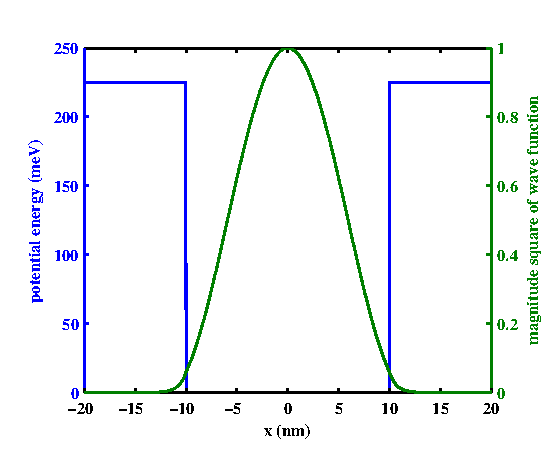
\includegraphics[width=0.7\textwidth]{./Pictures/wave1.eps}\\
  \caption{势函数以及第一能级波函数振幅的平方}
  \label{fig_wave1}
\end{figure}

\begin{figure}[!htb]
  \centering
  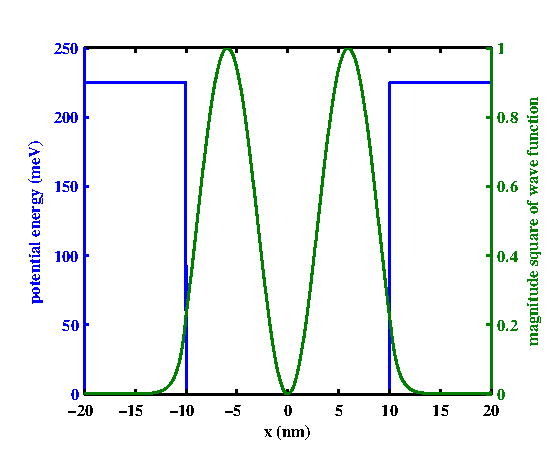
\includegraphics[width=0.7\textwidth]{./Pictures/wave2.eps}\\
  \caption{势函数以及第二能级波函数振幅的平方}
  \label{fig_wave2}
\end{figure}

\begin{figure}[!htb]
  \centering
  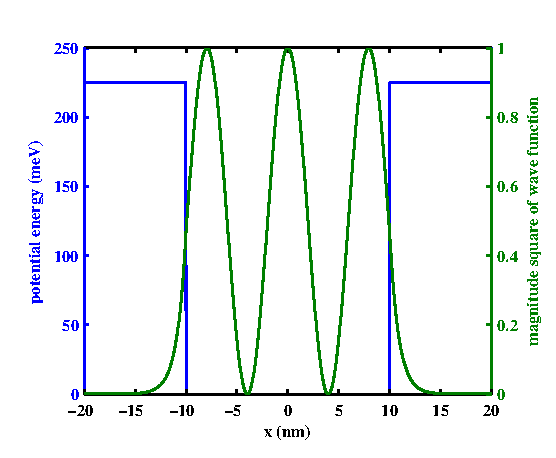
\includegraphics[width=0.7\textwidth]{./Pictures/wave3.eps}\\
  \caption{势函数以及第三能级波函数振幅的平方}
  \label{fig_wave3}
\end{figure}

\begin{figure}[!htb]
  \centering
  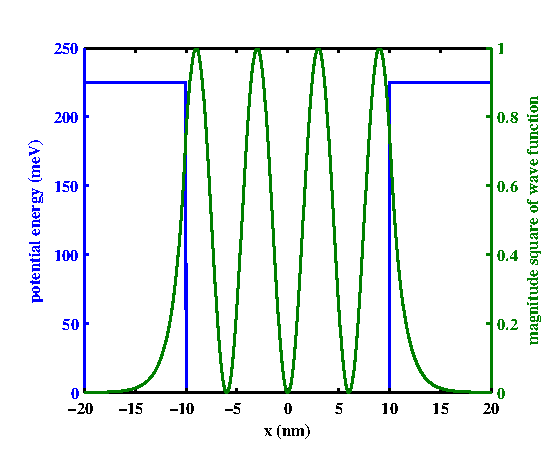
\includegraphics[width=0.7\textwidth]{./Pictures/wave4.eps}\\
  \caption{势函数以及第四能级波函数振幅的平方}
  \label{fig_wave4}
\end{figure}

\section{扩散模型}

Interdiffusion of atoms across the heterointerface alters the composition profile across the QW structure. Mathematical models are needed to describe and calculate the changes in the composition profile as a function of the duration of interdiffusion. In the section, we adopt the notation $A_{x}B_{1-x}C_{y}D_{1-y}$ to denote the chemical formula of a III-V semiconductor material, where A and B represent the Group III atoms, and C and D represent the Group V atoms respectively. After interdiffusion the mole fractions of Group III and V atoms are function of position along the direction of crystal growth (the $z$-direction) and are denoted by $w(z)$ and $v(z)$.

The diffusion process is usually described by the Fick's Second Law in the direction of crystal growth

\begin{equation}
  \frac{\partial{C}}{\partial{t}}=D\frac{\partial^2{C}}{\partial{z^2}}
\end{equation}

where $C$ denotes the concentration of the atoms and $D$ is the diffusion coefficient. The diffusion coefficient of the atoms is usually assumed to be identical in the quantum well. The interdiffusion process is characterized by a diffusion length $L_d$, which is defined as $L_d=\sqrt{Dt}$, where $D$ is the diffusion coefficient and $t$ is the annealing time of the thermal processing. Consider a single $In_{wx}Ga_{1-wx}As_{wy}P_{1-wy}/In_{bx}Ga_{1-bx}As_{by}P_{1-by}$ quantum well, the composition profile of In and As in this QW after interdiffusion are given by

\begin{eqnarray}
    w(z)&=&wx-\frac{bx-wx}{2} \notag\\
        &&\times \biggr[2-\textrm{erf}\biggr(\frac{L_z+2z}{4L_d^{III}}\biggr)
        -\textrm{erf}\biggr(\frac{L_z-2z}{4L_d^{III}}\biggr)\biggr]
\end{eqnarray}

\begin{eqnarray}
    v(z)&=&wy-\frac{by-wy}{2} \notag\\
        &&\times \biggr[2-\textrm{erf}\biggr(\frac{L_z+2z}{4L_d^{V}}\biggr)
        -\textrm{erf}\biggr(\frac{L_z-2z}{4L_d^{V}}\biggr)\biggr]
\end{eqnarray}

In this case, interdiffusion can occur on both group III and V sublattices, which are characterized by their diffusion lengths $L_d^{III}$ and $L_d^V$, respectively. The diffusion length ratio, i.e., $k=L_d^V/L_d^{III}$, depends on the details of interdiffusion process and is still an open question which requires further studies.


\section{能带结构计算}

\begin{equation}
    \label{V_c}
    V_c(z)
        = Q_c Eg(z) - (1-Q_c)S_\perp(z)
\end{equation}

\begin{equation}
    \label{V_HH}
    V_{HH}(z)
        = (1-Q_c)[Eg(z) - S_\perp(z)] + S_\parallel(z)
\end{equation}

\begin{eqnarray}
    \label{V_LH}
    V_{LH}(z)&=& (1-Q_c)[Eg(z) - S_\perp(z)] \notag\\
    && +0.5[S_\parallel(z) + \Delta_0(z)] \notag\\
    && -0.5 \sqrt{9S_\parallel^2(z)-2S_\parallel^2(z)\Delta_0(z)+\Delta_0^2(z)}
\end{eqnarray}

The calculation of the potential energy has take consideration the strain effect of the quantum well materials by Equation \ref{S_perp}-\ref{epsilon}. All the material parameters for the numerical calculation can be obtained from Table \ref{parametertable}.

\begin{equation}
    \label{S_perp}
    S_\perp(z)
        = -2a_v(z)[1-\frac{C_{12}(z)}{C_{11}(z)}] \epsilon(z)
\end{equation}

\begin{equation}\label{S_parallel}
    S_\parallel(z)
        = -b(z)[1+\frac{2C_{12}(z)}{C_{11}(z)}] \epsilon(z)
\end{equation}

\begin{equation}\label{a_v}
    a_v(z)
        = -\frac{1}{3}[C_{11}(z)+2C_{12}(z)] \frac{dEg}{dp}(z)
\end{equation}

\begin{equation}\label{epsilon}
    \epsilon(z)
        = \frac{a_{InP}(z)-a(z)}{a(z)}
\end{equation}

{
\begin{table}[!htb]
    \zihao{6}
    \caption{室温条件下(300K)InGaAsP量子阱材料的参数}
    \centering
    \label{parametertable}
    \begin{tabular}{llll}
        \hline
        \hline
        符号 & 参数 & $In_{x}Ga_{1-x}As_{y}P_{1-y}$ & 单位\\
        \hline
        $Q_c:Q_v$ & 能带偏移分裂比 & $0.6:0.4$ & $-$\\
        $E_g(z)$ & 禁带宽度 & $1.35-1.17y+0.668(1-x)-0.069y(1-x)+0.18y^2$ & eV\\
                                  && $+0.03(1-x)y^2+0.758(1-x)^2-0.322y(1-x)^2$ &\\
        $\Delta_0(z)$ & 自旋轨道分裂 & $0.34(1-x)y+0.43xy+0.10(1-x)(1-y)+0.10x(1-y)$ & eV\\
        $m_e$ & 电子质量 & $0.91095\times10{-30}$ & kg\\
        $m_c^*(z)$ & 电子有效质量 & $0.0632(1-x)y+0.0213xy+0.17(1-x)(1-y)+0.077x(1-y)$ & $m_e$\\
        $m_{\perp HH}^*(z)$ & 垂直方向 & $0.5(1-x)y+0.41xy+0.54(1-x)(1-y)+0.12x(1-y)$ & $m_e$\\
                            & 重空穴有效质量 &&\\
        $m_{\perp LH}^*(z)$ & 垂直方向& $0.088(1-x)y+0.024xy+0.16(1-x)(1-y)+0.12x(1-y)$ & $m_e$\\
                            & 轻空穴有效质量&&\\
        $m_{\parallel HH}^*(z)$ & 水平方向 & $0.11(1-x)y+0.031xy+0.19(1-x)(1-y)+0.15x(1-y)$ & $m_e$\\
                                & 重空穴有效质量 &&\\
        $m_{\parallel LH}^*(z)$ & 水平方向 & $0.23(1-x)y+0.082xy+0.34(1-x)(1-y)+0.29x(1-y)$ & $m_e$\\
                                & 轻空穴有效质量 &&\\
        $a(z)$ & 晶格常数 & $0.56533(1-x)y+0.60584xy+0.54512(1-x)(1-y)+0.58688x(1-y)$ & nm\\
        $C_{11}(z)$ & 弹性刚度常数 & $11.8(1-x)y+8.329xy+14.12(1-x)(1-y)+10.22x(1-y)$ & $10^{11}dyn/cm^2$\\
        $C_{12}(z)$ & 弹性刚度常数 & $5.38(1-x)y+4.526xy+6.253(1-x)(1-y)+5.76x(1-y)$ & $10^{11}dyn/cm^2$\\
        $dE_g/dP(z)$ & 水静压系数 & $11.5(1-x)y+10.0xy+11.0(1-x)(1-y)+8.5x(1-y)$ & $10^{-6}eV/bar$\\
        $b(z)$ & 剪切形变势能 & $-1.7(1-x)y-1.8xy-1.5(1-x)(1-y)-2.0x(1-y)$ & eV\\
        \hline
        \hline
    \end{tabular}
\end{table}
}

To show the validity of the theoretical model, I adopt the data by Nanyang Technology University with the same method of argon plasma-induced QWI \cite{redshift}. The layer structure of samples used in the experiment is shown in Table \ref{RedShiftSample}. Figure \ref{ex_redshift} shows the PL spectra of one InP cap sample before plasma exposure and after plasma exposure followed by several rapid thermal annealing (RTA) process. The result shows that after argon plasma exposure, both the blueshift and redshift of the bandgap can be obtained by controlling the temperature of RTA.

\begin{table}[!t]
    \zihao{5}
    \caption{The layer structure for the undoped InGaAsP/InP single quantum well}
    \centering
    \label{RedShiftSample}
    \begin{tabular}{cccc}
        \hline
        \hline
        No. & Composition & Thickness(nm) & Layer\\
        \hline
        5 & $In_{0.53}Ga_{0.47}As$ & 500 & Buffer/cap\\
        4 & InP & 500 & Barrier/cap\\
        3 & $In_{0.71}Ga_{0.29}As_{0.61}P_{0.39}$ & 3.5 & Well\\
        2 & InP & 300 & Barrier\\
        1 & InP & $-$ & substrate\\
        \hline
        \hline
    \end{tabular}
\end{table}

\begin{figure}[!t]
    \centering
    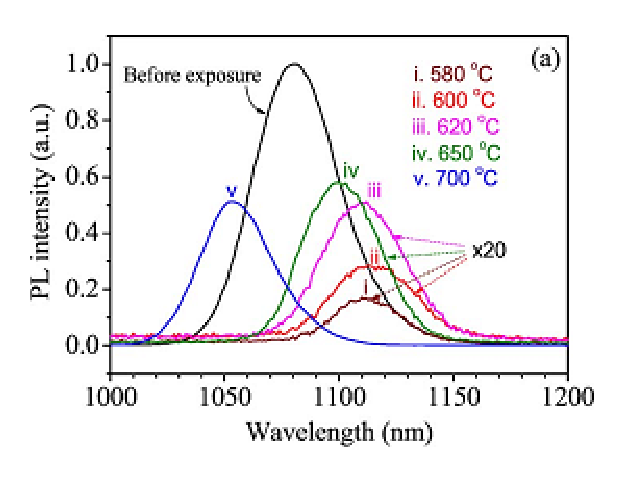
\includegraphics[width=0.7\textwidth]{./Pictures/exp_red.eps}
    \caption{PL spectra for one InP cap sample before plasma exposure and after plasma exposure followed by annealing at (i) 580$^\circ$C, (ii) 600$^\circ$C, (iii) 620$^\circ$C, (iv) 650$^\circ$C, (v) 700$^\circ$C.}
    \label{ex_redshift}
\end{figure}

To interpret the above observations of bandgap modification, the wavelength shift of the interdiffused QW structure was calculated using my theoretical model. Figure \ref{my_redshift} shows the calculated PL peak wavelength shift as a function of group III diffusion length under different k parameters. It can be seen that, in this QW structure, an observable redshift can be obtained only when k$<$0.63 roughly; i.e., the group III sublattice must interdiffuse about twice as fast as the group V sublattice.

\begin{figure}[!t]
    \centering
    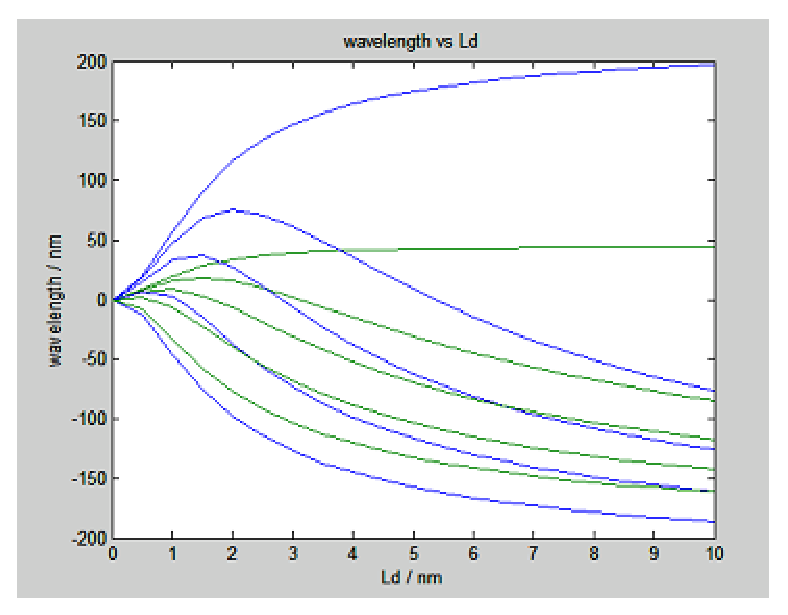
\includegraphics[width=0.7\textwidth]{./Pictures/red.eps}
    \caption{The calculated wavelength shift of the ground state transition as a function of the group III diffusion length under different k parameters.}
    \label{my_redshift}
\end{figure}

\section{材料的其他参数的计算}

量子限制斯塔克效应。

\begin{equation}
    \label{QCSE}
    \frac{-h^2}{2}
    \frac{d}{dz}
    \frac{1}{m_\perp^*(z)}
    \frac{d\varphi(z)}{dz}
    +[V(z)+zeE]\varphi(z)
        = E\varphi(z)
\end{equation}


增益。

\begin{eqnarray}
    g(\hbar\omega) &=& \frac{2 m_r \omega}{n_{eff} c \varepsilon_0 \pi \hbar^2 L_z}
        \sum_{n,m} \int_0^\infty dE_\parallel |e\cdot M_{cv}(E_\parallel)|^2 \notag\\
    && \times \frac{\frac{\hbar}{\pi \tau_{in}}}
        {(E_{en}-E_{hm}+E_\parallel-\hbar\omega)^2+(\frac{\hbar}{\pi \tau_{in}})^2} \notag\\
    && \times [f_c^n(E_\parallel)-f_v^m(E_\parallel)]
\end{eqnarray}

折射率。

\begin{eqnarray}
    \Delta n(\hbar\omega) &=& \frac{m_r}{n_{eff} c \varepsilon_0 \pi \hbar^2 L_z}
        \sum_{n,m} \int_0^\infty dE_\parallel |e\cdot M_{cv}(E_\parallel)|^2 \notag\\
    && \times \frac{E_{en}-E_{hm}+E_\parallel-\hbar\omega}
        {(E_{en}-E_{hm}+E_\parallel-\hbar\omega)^2+(\frac{\hbar}{\pi \tau_{in}})^2} \notag\\
    && \times [f_c^n(E_\parallel)-f_v^m(E_\parallel)]
\end{eqnarray}


%%%%%%%%%%%%%%%%%%%%%%
\chapter{KrF准分子激光器照射实现量子阱混杂技术的工艺研究}



%%%%%%%%%%%%%%%%%%%%%%

\chapter{量子阱混杂技术在集成光子回路中的应用}

\section{V型腔激光器}

随着密集波分复用(DWDM)技术的广泛使用,波长敏捷型光子集成回路变得越来越重要。波分复用技术通过在一路光纤中传输多路光信号的方法,增加了网络的带宽。国际通信联盟(ICU)制定了WDM的基本规则。现在的光信道的间隔为100GHz或0.8纳米,未来将会变成50GHz或25GHz。要实现WDM,就需要激光器覆盖ICU规定的每个信道。想要覆盖这么多的信道,使用大范围可调谐激光器是一个明智的选择。

现在人们在实验室已经制造出了很多种大范围可调谐激光器。其中一种就是V型腔激光器。V型腔激光器的示意图如图\ref{fig_vccl}所示。其主要部分包含两个长度不同的光学谐振腔,一个耦合相位为 180°的半波耦合器以及一个波长调谐区。另外在V字型的闭合端(图\ref{fig_vccl}中右端)有一个耦合器,V字型的开口端(图\ref{fig_vccl} 中左端)为一个多模耦合器(MMI)。

\begin{figure}[!htb]
  \centering
  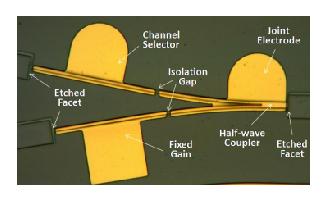
\includegraphics[width=0.7\textwidth]{./Pictures/vccl.eps}\\
  \caption{V型腔激光器的光学显微镜图\cite{jin201116-VCCL}}
  \label{fig_vccl}
\end{figure}

其中第一个光学谐振腔由一段光波导以及两端的深刻蚀反射槽构成,该段光学波导上面镀有一段电极用来注入电流以提供激光器谐振所需的增益,我们称之为固定增益腔(Fix Gain Cavity)。第二个光学谐振腔由两段光学波导以及两端的深刻蚀反射槽构成,其中一段波导提供增益,另一段波导为无源波导,可以通过注入电流来改变其光学长度从而来调谐激光器的工作波长,因此称之为信道选择腔(Channel Selector Cavity)。两段波导中间由一个浅刻蚀槽隔开。在V字型的闭合端,两个谐振腔中间由一个耦合相位为 180°的半波耦合器相连,通过设计优化两个腔之间的耦合系数可以使得整个复合耦合腔激光器实现高的边模抑制比和良好的单模特性。另外波长调谐区离耦合区较远,使得其折射率的改
变几乎不影响两个谐振腔之间的耦合系数。左端的MMI 耦合器用来将两根波导的输出光耦合到一跟波导,同时可以通过调节一个臂的注入电流来切换光输出的端口,用以做空间光开光。

为了实现激光器工作波长的数字式调谐,固定增益腔的长度要根据激光器的工作波长来确定,使得固定增益腔的谐振频率的间隔与预先要求的频率间隔一致,例如根据ITU的规定,各个通信波长的间隔为200GHz、100GHz或者50GHz等。谐振腔的频率间隔可由下式确定:
\begin{equation}
  \Delta f = \frac{c}{2 n_g L}
\end{equation}

其中$c$是真空中的光速,$n_g$是波导的有效群折射率,$L$是固定增益腔的长度。

同样,第二个谐振腔(信道选择腔)的频率间隔$\Delta f ^\prime$由式\ref{eqa_Daltafprime}决定:
\begin{equation}\label{eqa_Daltafprime}
  \Delta f ^\prime= \frac{c}{2 n_g^\prime L^\prime} = \frac{c}{2 (n_a L_a + n_b L_b)}
\end{equation}

其中$L_a$和$L_b$分别为信道选择腔的增益区以及波长调谐区的长度,同样$n_a$和$n_b$分别为信道选择腔的增益区以及波长调谐区的有效群折射率。$L^\prime=L_a+L_b$是信道选择腔的总长度,$n_g^\prime=(n_a L_a + n_b L_b)/L^\prime$是信道选择腔的平均有效群折射率。

信道选择腔的频率间隔$\Delta f ^\prime$选择为与固定增益腔的频率间隔$\Delta f$有一个微小的差别,这使得在工作物质的增益窗口内,两者只有一个谐振峰恰好重合(如图\ref{fig_Deltaf}所示)。两个谐振腔相邻的互相重合的谐振峰之间的间隔为组合腔的自由光谱范围(FSR),其大小由式\ref{eqa_Daltafc}决定。为了避免两个波长同时被激发,$\Delta f_c$一般来讲必须大于激光器工作物质增益窗口的宽度。
\begin{equation}\label{eqa_Daltafc}
  \Delta f_c = \frac{\Delta f \Delta f^\prime}{|\Delta f-\Delta f^\prime|}
\end{equation}
\begin{figure}[!htb]
  \centering
  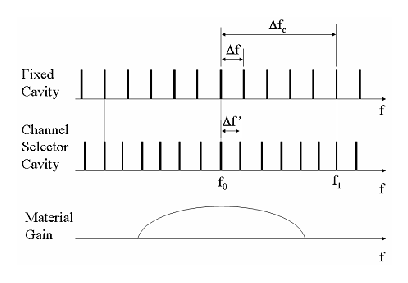
\includegraphics[width=0.7\textwidth]{./Pictures/deltaf.eps}\\
  \caption{固定增益腔和信道选择腔的谐振频率位置关系的示意图,以及激光工作物质的增益光谱曲线}
  \label{fig_Deltaf}
\end{figure}

固定增益腔以及信道选择腔的谐振频率分别为:
\begin{equation}
  f = \frac{mc}{2nL}
\end{equation}
\begin{equation}
  f^\prime = \frac{m^\prime c}{2n^\prime L^\prime}
\end{equation}
其中$m$和$m^\prime$都是整数,$n$和$n^\prime$分别为两个腔的平均有效折射率,$L$和$L^\prime$ 分别为两个腔的长度。信道选择腔的谐振频率$f^\prime$可以通过改变波长调谐区的折射率$n_b$从而改变整个腔的有效折射率$n^\prime$而改变。频率调谐量由下式决定:
\begin{equation}
  \frac{\delta f^\prime}{f^\prime} = -\frac{\delta n^\prime}{n^\prime}=-\frac{\delta n_b L_b}{n_b L^\prime}
\end{equation}

由于激光器的工作频率为固定增益腔与信道选择腔谐振峰重合的频率,因此$|\Delta f-\Delta f^\prime|$一个较小的变化将会导致激光器工作频率跳变一个信道。因此,激光器工作频率的改变量被放大了一个因子$\Delta f/|\Delta f-\Delta f^\prime|$,即:
\begin{equation}
  \delta f = \frac{\Delta f}{|\Delta f-\Delta f^\prime|} \delta f^\prime
\end{equation}

这种效应称作为游标效应。取样光栅(Sample Grating ,SG) 、超结构光栅(Super Structure Grating,SSG)也是利用类似的原理,但是取样光栅,超结构光栅的频率间隔是由光栅的调制周期决定,而且通常至少需要10个周期以上,为了获得同样的频率间隔,取样光栅超结构光栅的器件长度通常为V 型腔的20倍左右。

鉴于通常的ITU 标,假设$\Delta f=100GHz$,$\Delta f^\prime=90GHz$,则激光器工作频率的调节范围与仅靠调节折射率相比扩大了10倍。在上述数据下,设波导的有效群折射率为3.215,则固定增益腔以及信道选择腔的长度分别为:$L=466.24\mu m$,$L^\prime=518.31\mu m$,其长度与传统的DFB以及法布里- 珀罗激光器相当。相比之下,取样光栅、超结构光栅DBR激光器,由于受到器件长度以及损耗的限制,通常的信道间隔至少为600GHz,而对于通常的密集波分复用系统(DWDM)信道间隔一般为50GHz~200GHz,很难实现完全的数字式调谐。对于V型耦合腔宽带可调谐激光器,则完全不受此限制,并且利用深刻蚀槽做反射面技术,通过全息平版照相(photolithographic)技术可以精确控制激光器谐振腔的长度。激光器工作波长与ITU标准的些许偏离可以由微调固定腔的注入电流以及温度调谐来补偿。

\section{电调谐与热调谐的区别}

尽管V型腔激光器已经在InP和GaAs材料上同时取得了成功,但是他们距离实际商业应用还有很长的路要走。在光通信领域中,为了得到更快的速度,我们常常会使用尽可能快的调制器,例如电吸收调制器可以将调制速度提升到40Gbps(文献?),甚至使用行波电极做到100Gbps(?)。除了提升同一个波长信号的调制速度,还要提升不同波长信号之间的切换速度。2012年,浙江大学的郭山溧等人测试了V型腔激光器的波长切换速度\cite{guo2012experimental}。他们所测试的激光器波长调谐曲线如图\ref{fig_gsl_tuning}所示。在波长调谐电流大于45mA的情况下,激光器的输出波长随着电流的增加而增加,这与之前的所有文章中的结果是一致的,也就是热调谐。而当调谐电流小于20mA时,激光器的输出波长随着电流的增加而减小,这与之前的情况刚好相反,这主要是载流子注入调谐,也就是电调谐在起作用。而在20mA和45mA之间的部分,波长没有发生跳变,也就是电调谐和热调谐的作用刚好相互抵消。然后,他们选择了其中的四个波长,如表\ref{tab_4wavelength}所示。其中,通道A和通道B之间的切换时间通过光外差方法测试得到仅有500ps,也就是相当于2G的速度。而通道3和通道4之间的切换时间通过光滤波器方法测试得到有20us,也就是相当于50k的速度。显然,热调谐的速度远远小于电调谐的速度。同时,电调谐需要的电流远小于热调谐的电流,这样还可以减小整个激光器的功耗。在实际的光通信应用中,我们需要的是电调谐的V型腔激光器。

\begin{figure}[!htb]
    \centering
    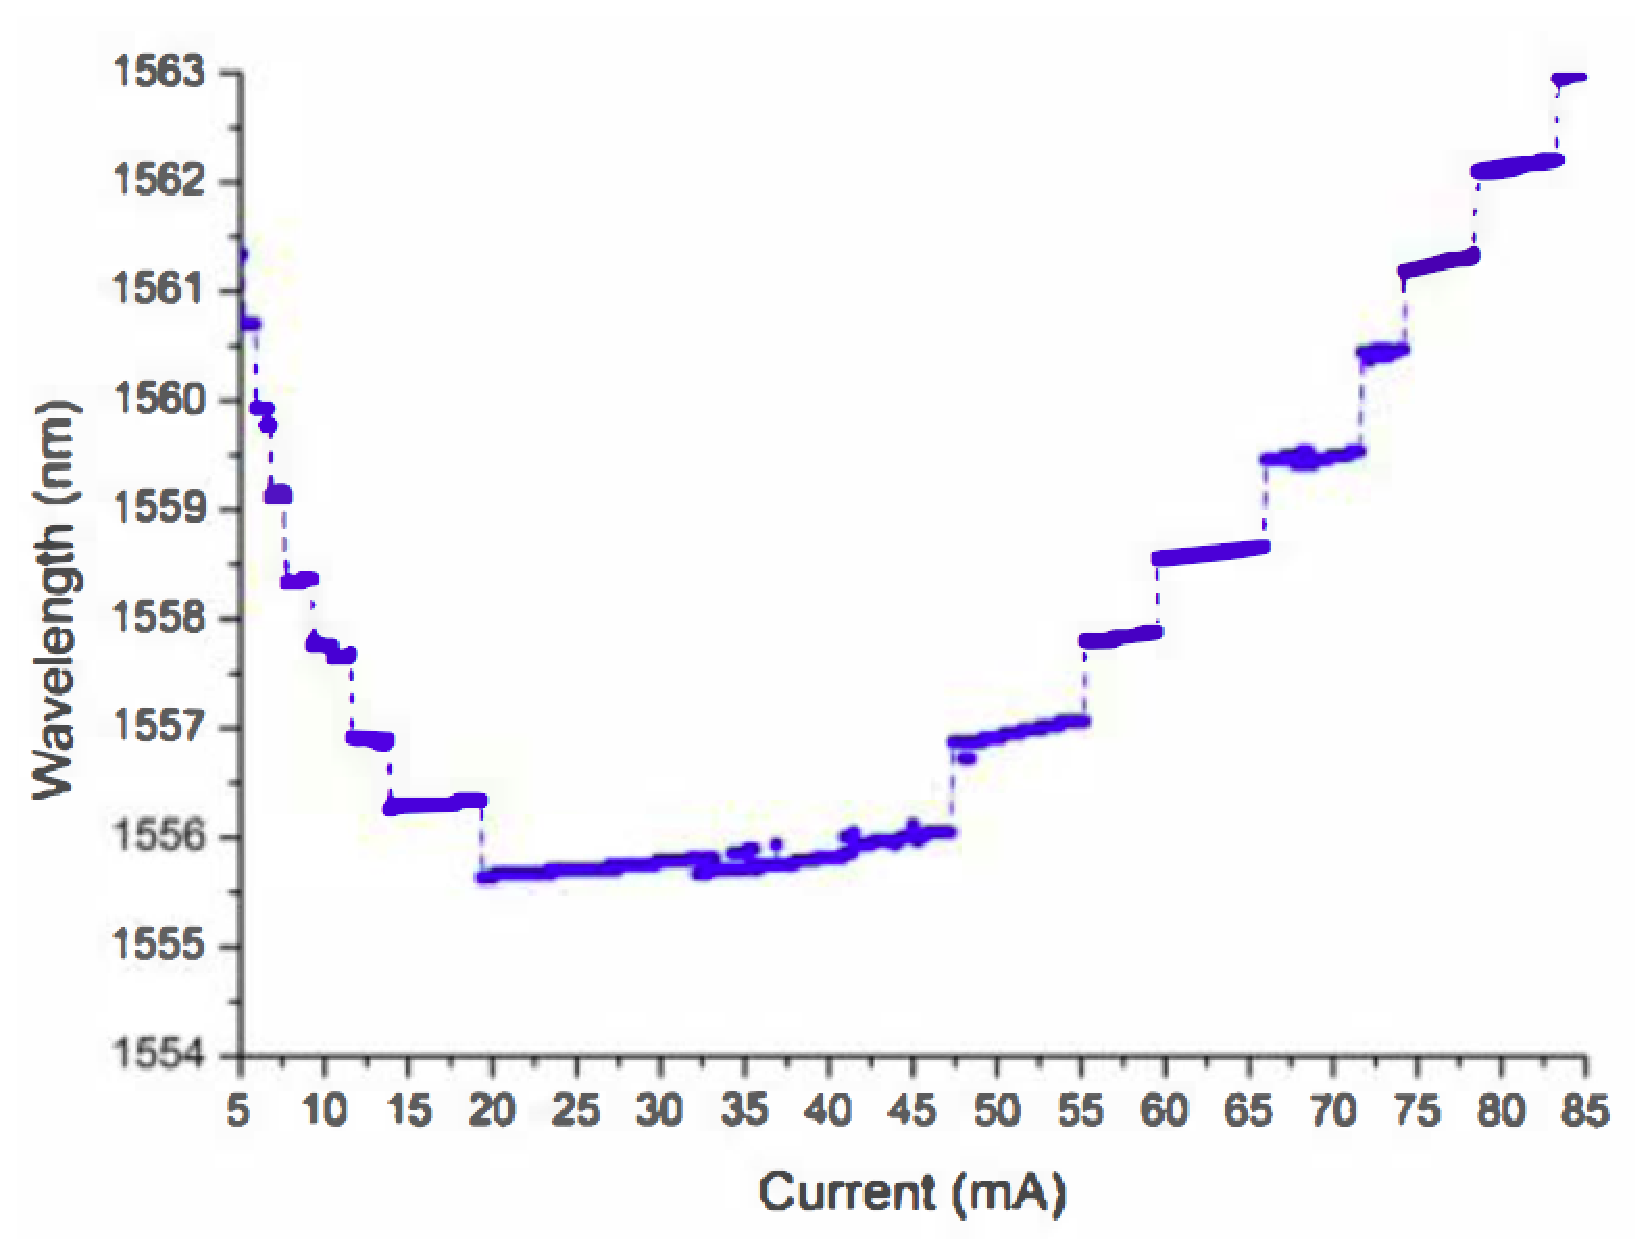
\includegraphics[width=0.7\textwidth]{./Pictures/GSL_tuning.eps}
    \caption{V型腔激光器的波长调谐曲线}
    \label{fig_gsl_tuning}
\end{figure}

\begin{table}[!t]
    \zihao{5}
    \caption{测试的4个波长以及对应的电流}
    \centering
    \label{tab_4wavelength}
    \begin{tabular}{ccccc}
        \hline
        \hline
         & 通道A & 通道B & 通道C & 通道D\\
        \hline
        电流(mA) & 17 & 25 & 	39 & 49\\
        波长(nm) & 1556.33 & 1555.70 & 1555.88 & 1556.67\\
        \hline
        \hline
    \end{tabular}
\end{table}

然而,要实现电调谐的V型腔激光器并没有那么简单。在郭山溧的文章中,我们可以看到电调谐得到的波长通道仅有8个,而且他们的边模抑制比特性甚至由于太不好而没有给出。所以,我们希望将电调谐和热调谐达到平衡的流量值,尽可能往大电流的方向上移动,同时能保持输出光谱的边模抑制比在35dB以上。其中一种方法就是将V型腔的调谐腔处理成无源腔。2003年,加州大学圣芭芭拉校区的Erik J. Skogen等人研究了量子阱混杂的蓝移对载流子注入调谐的范围影响,如图\ref{fig_qwi_tuning}所示。显然,蓝移最大的情况下能得到的载流子注入调谐的范围也是最大的。这说明了我们需要在V型腔的调谐腔上做出尽可能大的蓝移,同时不改变材料的其他特性。

\begin{figure}[!htb]
    \centering
    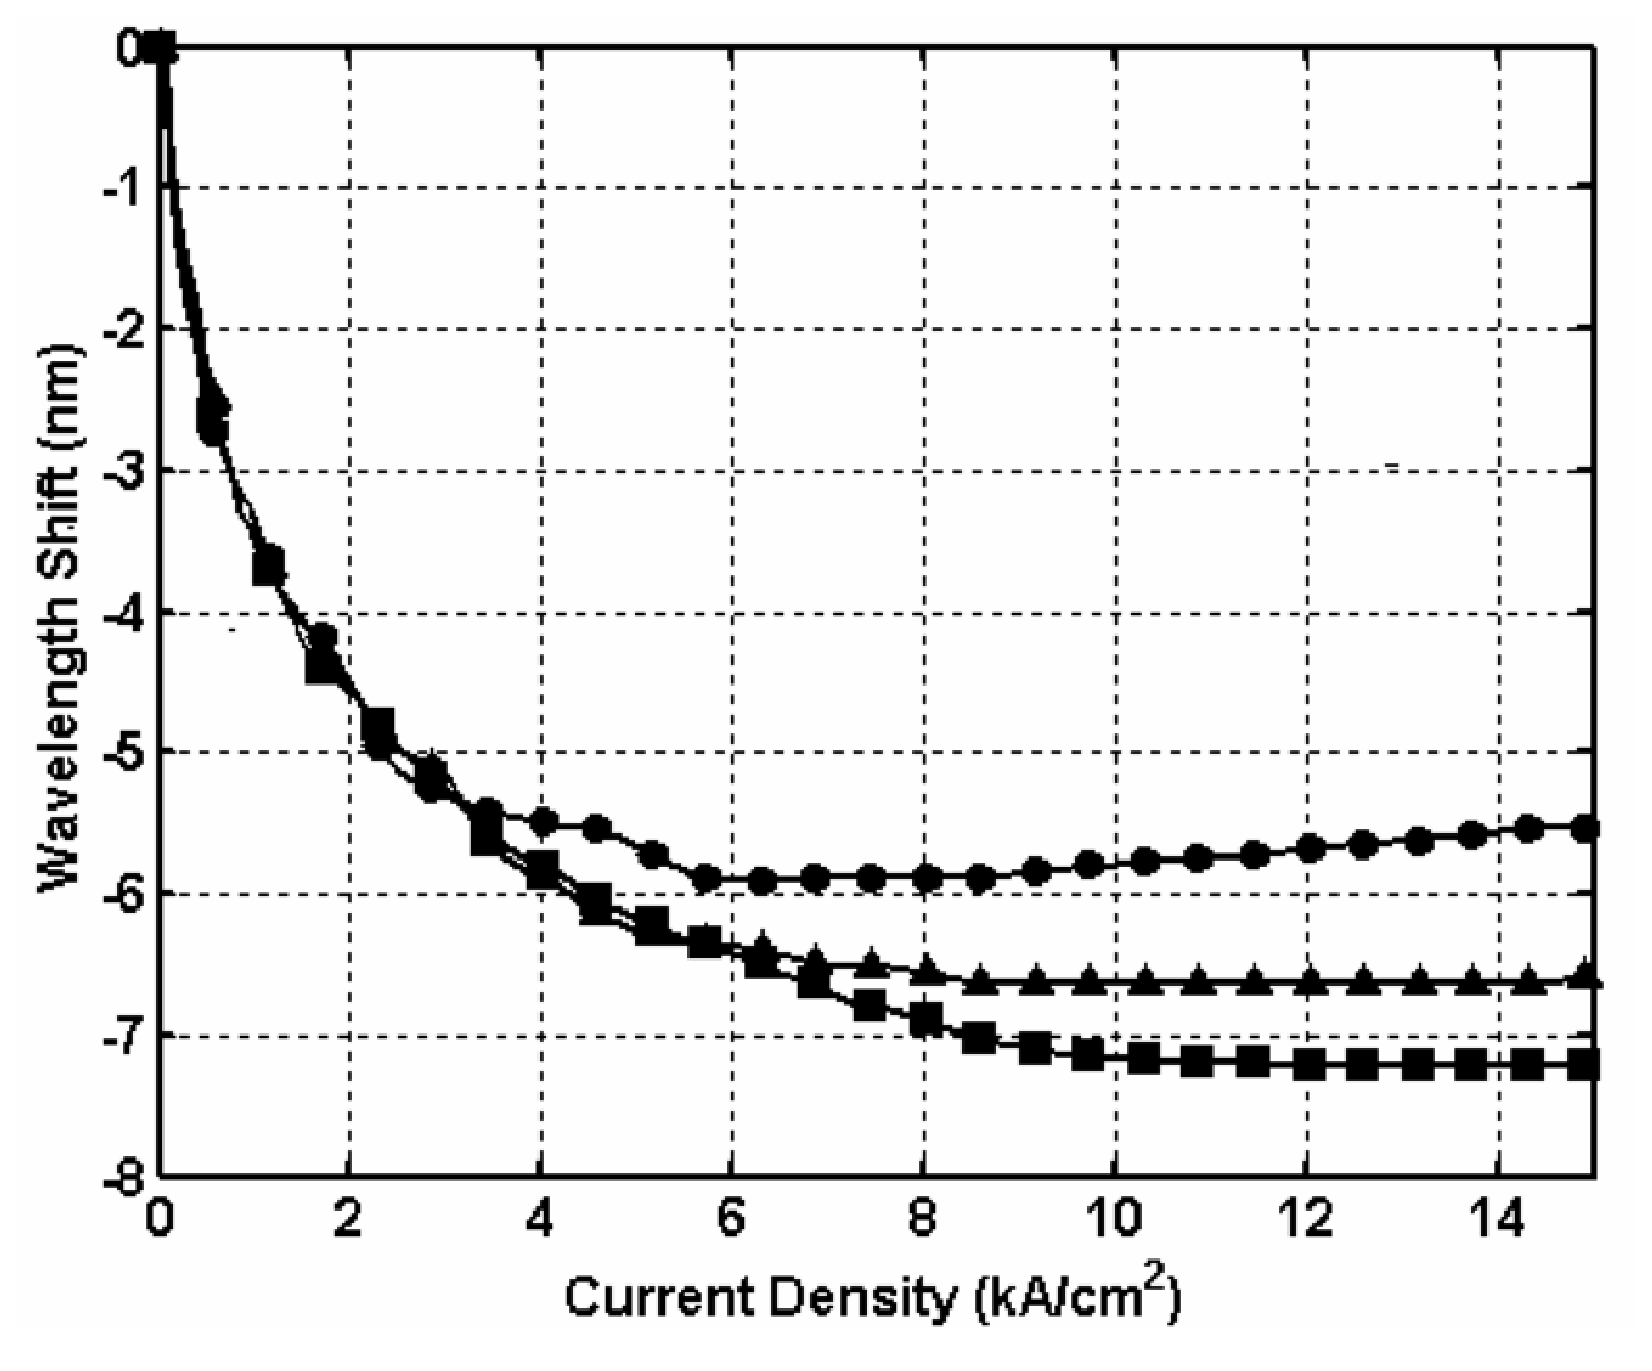
\includegraphics[width=0.7\textwidth]{./Pictures/qwi_tuning.eps}
    \caption{量子阱混杂的蓝移大小(圆形1475nm,三角形1446nm,方形1423nm)对载流子注入调谐大小的影响}
    \label{fig_qwi_tuning}
\end{figure}


\section{包含量子阱混杂技术的V型腔激光器的制作过程}

包含量子阱混杂的V型腔激光器的AutoCAD设计图如图\ref{fig_vccl_design}所示。

\begin{figure}[!htb]
    \centering
    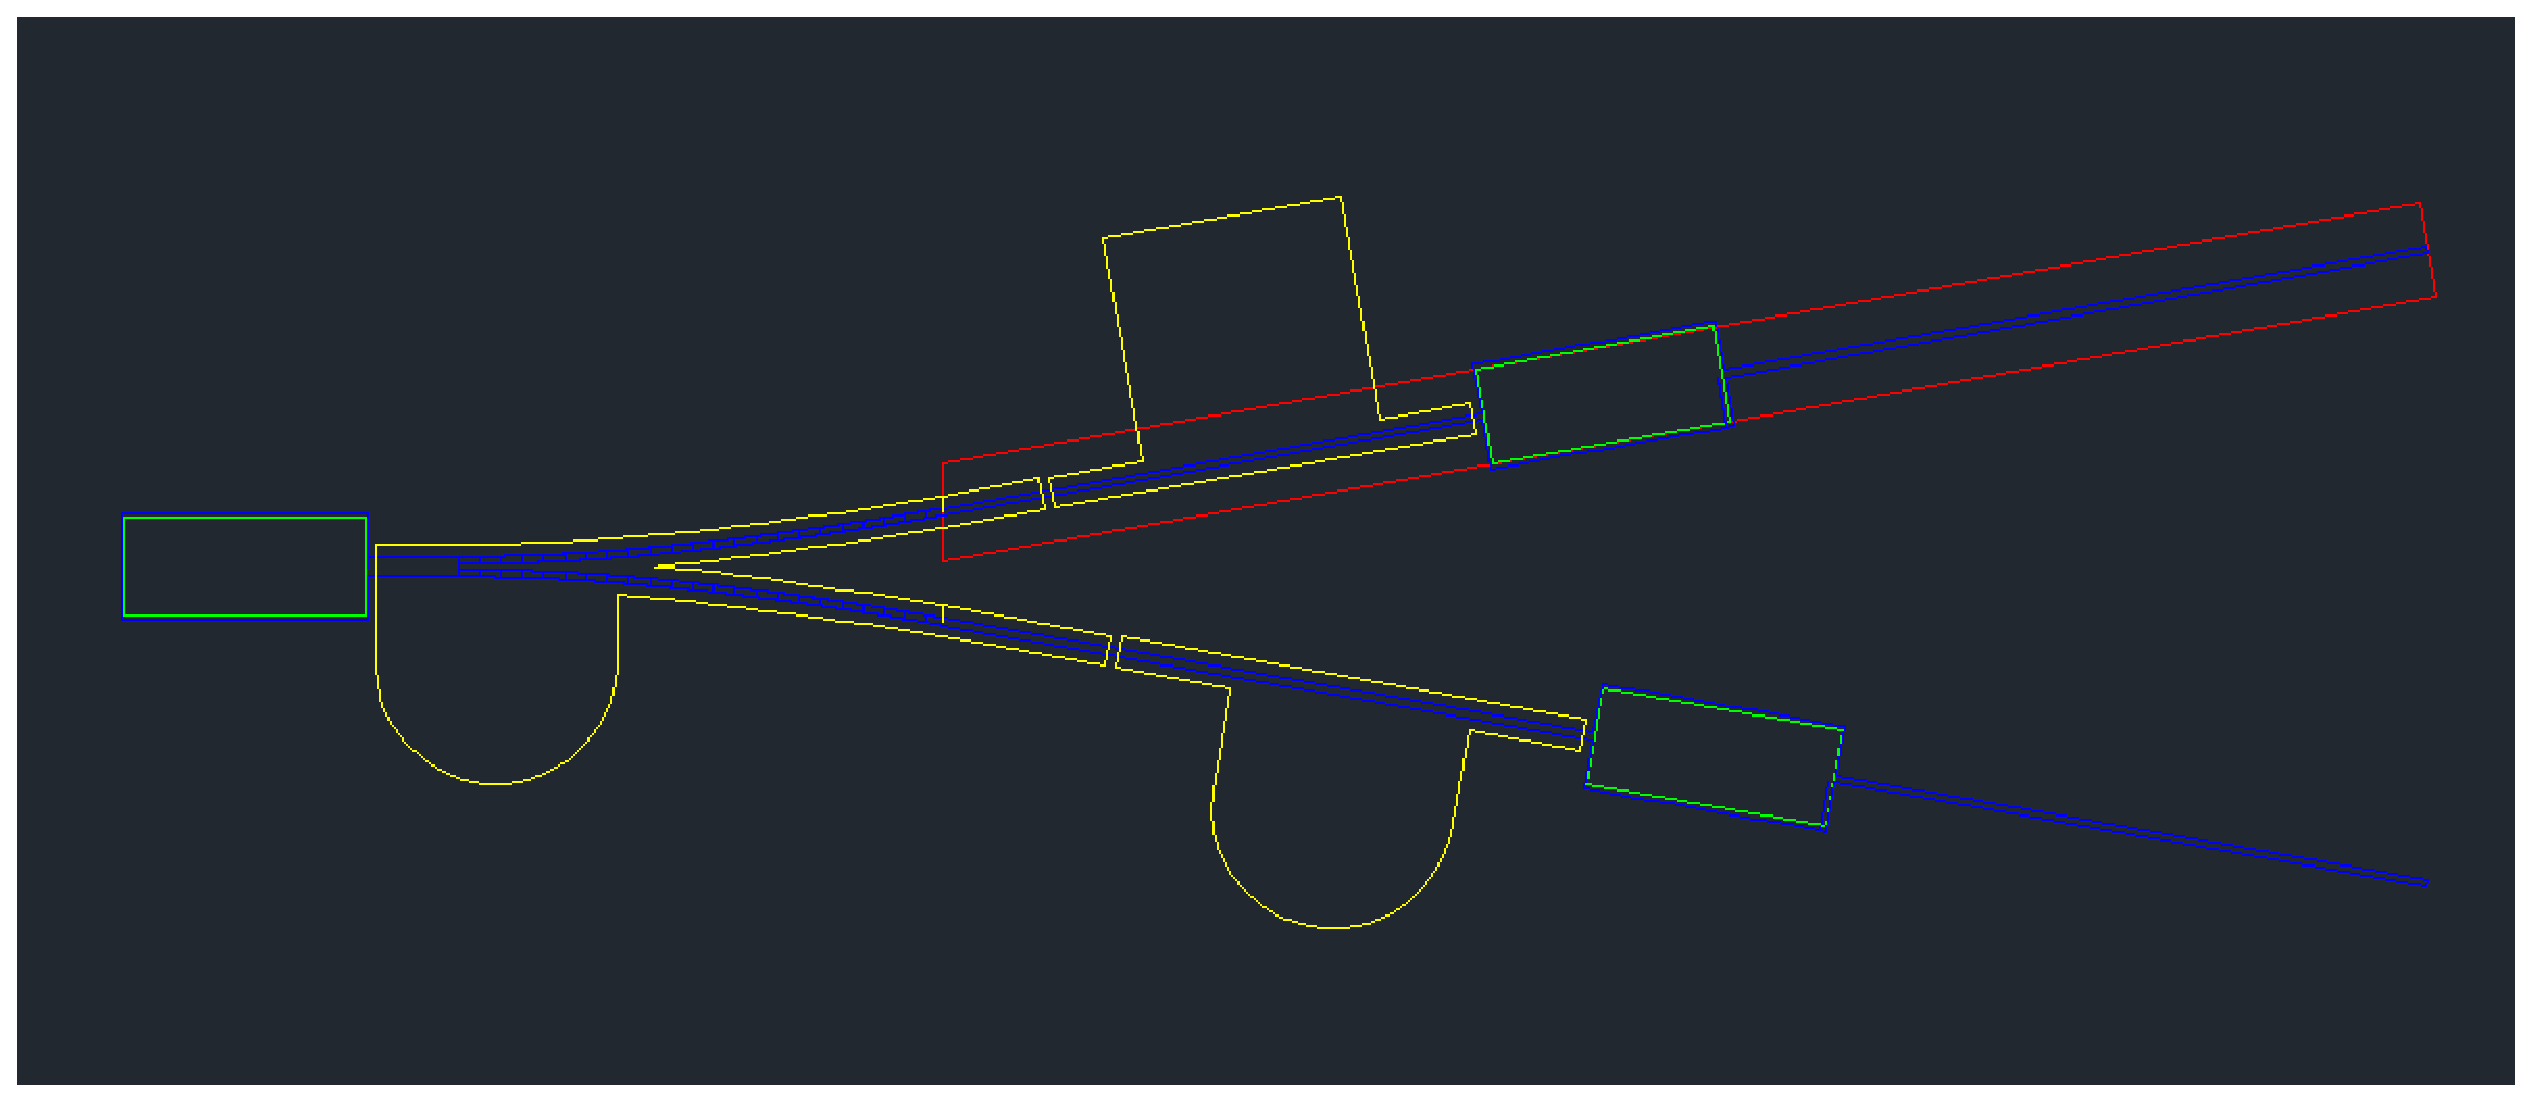
\includegraphics[width=0.7\textwidth]{./Pictures/vccl_design.eps}
    \caption{包含量子阱混杂的V型腔激光器的AutoCAD设计图}
    \label{fig_vccl_design}
\end{figure}


\section{测试结果与分析}

%%%%%%%%%%%%%%%%%%%%
\chapter{总结和展望}

\section{本文总结}

\section{本文展望}

\ZJUbackmatter
%%%%%%%%%%%%%%%%%%%%%%%%%%%%%%
%% 参考文献
%%%%%%%%%%%%%%%%%%%%%%%%%%%%%%
\bibliographystyle{ieeetr}
\bibliography{thesisbib}

%%%%%%%%%%%%%%%%%%%%%%%%%%%%%%
%% 个人简历
%%%%%%%%%%%%%%%%%%%%%%%%%%%%%%
\begin{resume}
\begin{enumerate}
\item{1986年10月12日,出生于浙江省杭州市}
\item{2009年6月,在浙江大学信息工程光电系获得工学学士学位}
\item{2014年6月,在浙江大学光电系获得工学博士学位}
\end{enumerate}
\end{resume}

%%%%%%%%%%%%%%%%%%%%%%%%%%%%%%
%% 发表论文目录
%%%%%%%%%%%%%%%%%%%%%%%%%%%%%%
\begin{publications}
\begin{enumerate}
\item{Yuan Zhuang, \textbf{Xin Zhang}, Mohammad Kaleem and Jian-Jun He. "Large bandgap shift by UV excimer laser induced quantum well intermixing for photonic integration." Asia Communications and Photonics Conference and Exhibition. Optical Society of America, 2013.}
\item{Kaleem, Mohammad, et al. "UV laser induced selective-area bandgap engineering for fabrication of InGaAsP/InP laser devices." Optics and Laser Technology 51 (2013): 36-42.}
\item{Kaleem, Mohammad, \textbf{Xin Zhang}, and Jian-Jun He. "Bandgap engineering of InGaAsP/InP laser structure by argon plasma induced point defects." Communications and Photonics Conference (ACP), 2012 Asia. IEEE, 2012.}
\item{彭盛华, \textbf{张欣}, and 何建军. "氩等离子体诱导量子阱混合技术." 浙江大学学报 (工学版) 6 (2011): 015.}
\item{\textbf{Zhang, Xin}, and Jian-Jun He. "Optical loss of bandgap shifted InGaAsP/InP waveguide using argon plasma-enhanced quantum well intermixing." Advances in Optoelectronics and Micro/Nano-Optics (AOM), 2010 OSA-IEEE-COS. IEEE, 2010.}
\item{Shenghua Peng, \textbf{Xin Zhang} and Jian-Jun He. "Nitrogen plasma enhanced quantum well intermixing in InGaAsP/InP laser structure." Asia Communications and Photonics Conference and Exhibition. Optical Society of America, 2009.}
\item{何建军, \textbf{张欣}, 彭盛华. "一种量子阱混合方法." 中国发明专利CN101697341A}
\item{何建军, \textbf{张欣}, 彭盛华. "一种量子阱混杂方法." 中国发明专利CN101774540A}
\end{enumerate}
\end{publications}

\end{document}
